\documentclass[11pt]{article}
\usepackage{graphicx} % Required for inserting images
\linespread{1.2}
\usepackage[top=2cm, bottom=2cm, left=2cm, right=2cm, centering]{geometry}
\usepackage[]{hyperref}
\usepackage{tabularx}
\usepackage{tabularray}
\usepackage{amsmath}
\usepackage{amssymb}
\usepackage{bm}
\usepackage{bbm}
\usepackage{algorithm}
\usepackage{algpseudocode}
\usepackage{svg}
\usepackage{enumitem}
\usepackage{titlesec}
\usepackage[dvipsnames]{xcolor}
\usepackage{tikz}
\usepackage[breakable]{tcolorbox}
\appto{\bibsetup}{\raggedright}

\setlength\jot{10pt} % to increase space between equations

\tikzstyle{mybox} = [draw=NavyBlue, ultra thick, rectangle, rounded corners, inner sep=10pt, inner ysep=10pt, text width=0.90\textwidth, align=left] 
\tikzstyle{boxtitle} = [fill=NavyBlue, text=white, ultra thick, rectangle, rounded corners, inner sep=10pt, inner ysep=8pt, text width=0.90\textwidth]
\tikzstyle{boxsubtitle} = [fill=NavyBlue!80, text=white, ultra thick, rectangle, outer ysep=-2.5pt, inner sep=10pt, inner ysep=5pt, text width=0.90\textwidth,
path picture={
    \draw[NavyBlue, ultra thick] 
        (path picture bounding box.north west) -- (path picture bounding box.south west)
        (path picture bounding box.north east) -- (path picture bounding box.south east);
}]

\newcommand{\distribution}[3]{%
\noindent

\begin{center}
\begin{tikzpicture}
    \node[mybox](box){\rule{0pt}{50pt}\ignorespaces#3\unskip};
    \node (t) [boxtitle, anchor=north west] at (box.north west) {\textbf{#1}};
    \node[boxsubtitle, anchor=north west] at (t.south west) {\textbf{#2}};
\end{tikzpicture}
\end{center}
\vspace{-8pt}
}

\newcommand{\boxdefinition}[2]{%
\vspace*{1.0px}
\noindent

\begin{center}
\begin{tikzpicture}
    \node[mybox](box){\rule{0pt}{30pt}\ignorespaces#2\unskip};
    \node[boxtitle, anchor=north west] at (box.north west) {\textbf{#1}};
\end{tikzpicture}
\end{center}
\vspace{-2pt}
}

\newcommand{\separate}{\begin{center}\textcolor{NavyBlue}{\rule{16cm}{1mm}}\end{center}}
\newcommand{\E}{\mathbb{E}}
\newcommand{\indep}{\perp \!\!\! \perp}

\begin{document}

\begin{titlepage}
    \hrule
    \vspace{15pt}
    \begin{center}
        \Huge{\textbf{\Huge \textbf{Statistics for Data Science 24-25}} \\ Notes}\\
    \end{center}
    \vspace{15pt}
    \hrule
    \vfill
    \hrule
    \begin{center}
        \Large University of Pisa \\ M.Sc. in Data Science and Business Informatics
    \end{center}
\end{titlepage}

\tableofcontents
\clearpage

\section*{Probability}
\boxdefinition{Probability (on a finite sample space)}
{
    A probability function $P$ on a finite sample space assigns to each event $A \in \Omega$ a number $P(A) \in [0,1]$ such that
    \begin{itemize}
        \item $P(\Omega) = 1$;
        \item $P(A \cup B) = P(A) + P(B)$ if $A$ and $B$ are disjoint.
    \end{itemize}
    $P(A)$ is called probability that event $A$ occurs.
}
\boxdefinition{Probability (on an infinite sample space)}{
    A probability function $P$ on an infinite sample space assigns to each event $A \in \Omega$ a number $P(A)$ such that
    \begin{itemize}
        \item $P(\Omega) = 1$;
        \item $P(A_1 \cup A_2 \cup A_3 \cup \dots) = P(A_1) + P(A_2) + P(A_3) + \dots$ if $A_1, A_2, A_3, \dots$ are disjoint.
    \end{itemize}
}
Properties:
\begin{itemize}[itemsep=1pt]
    \item $P(A^c) = 1 - P(A)$
    \item $P(\emptyset) = 0$
    \item $P(A \cup B) = P(A) + P(B) - P(A \cap B)$
    \item $A \subseteq B \implies P(A) \leq P(B)$
\end{itemize}

\boxdefinition{Conditional probability}{
    The conditional probability of $A$ given $C$ is given by
    \begin{equation*}
        P(A|C) = \frac{P(A \cap C)} {P(C)}
    \end{equation*}
    provided $P(C) > 0$ (it is otherwise undefined).
}
A consequence of this definition is the \textbf{multiplication rule}: $P(A \cap C) = P(A|C) \cdot P(C) = P(C|A) \cdot P(A)$.
\boxdefinition{Law of total probability}{
    Let $C_1, C_2, \dots, C_n$ be a partition of $\Omega$ (i.e., they are disjoint and their union is $\Omega$). Then, given any event $A \in \Omega$, its probability can be computed as
    \begin{equation*}
        P(A) = P(A|C_1) \cdot P(C_1) + P(A|C_2) \cdot P(C_2) + \dots + P(A|C_n) \cdot P(C_n)
    \end{equation*}
}
\boxdefinition{Bayes' rule}{
    Let $C_1, C_2, \dots, C_n$ be a partition of $\Omega$ and $A$ be an event in $\Omega$. Then, the probability of $C_i$ given $A$ is given by
    \begin{equation*}
        P(C_i|A) = \frac{P(A|C_i) \cdot P(C_i)} {P(A|C_1) \cdot P(C_1) + P(A|C_2) \cdot P(C_2) + \dots + P(A|C_n) \cdot P(C_n)}
    \end{equation*}
}
Two events $A$ and $B$ are \textbf{independent} if $P(B) = 0$, or:
\begin{itemize}[itemsep=1pt]
    \item $P(A \cap B) = P(A) \cdot P(B)$, or, equivalently,
    \item $P(A|B) = P(A)$.
\end{itemize}
If $A$ and $B$ are independent, also any combination of their complements is independent. \\
In general, events $A_1, A_2, \dots, A_n$ are independent if for any subset $I \subseteq \{1, 2, \dots, n\}$:
\begin{equation*}
    P\left(\bigcap_{i \in I} A_i\right) = \prod_{i \in I} P(A_i)
\end{equation*}
This means that any possible subset of events in the collection is independent (since pairwise independence among individual events is not enough).

Two events $A$ and $B$ are \textbf{conditionally independent} given and event $C$ ($P(C) > 0$) if $P(B|C) = 0$, or $P(A|B \cap C) = P(A|C)$. Since conditional probability is a probability, the definition is identical to the one above but conditioned on $C$.
\separate
\section{Random variables}
A \textbf{discrete random variable} takes a finite number of values, or a countably infinite number of values. Each discrete r.v. is described by a probability mass function and a cumumlative distribution function.
\boxdefinition{Probability mass function (PMF)}{
    The PMF $p$ of a discrete random variable $X$ is a function $p: \mathbb{R} \rightarrow [0,1]$, defined by
    \begin{equation*}
        p(a) = P(X = a) \text{ for } -\infty < a < \infty
    \end{equation*}
}
A \textbf{continuous random variable} takes any value in a continuous range (finite or infinite). Each continuous r.v. is described by a probability density function and a cumulative distribution function.
\boxdefinition{Probability density function (PDF)}{
    A random variable $X$ is countinuous if for some function $f: \mathbb{R} \rightarrow \mathbb{R}$ and any numbers $a, b$, with $a < b$,
    \begin{equation*}
        P(a \leq X \leq b) = \int_a^b f(x) dx
    \end{equation*}
    where $f(x) \geq 0$ for all $x$ and $\int_{-\infty}^{\infty} f(x) dx = 1$. $f$ is called probability density function (PDF) of $X$.
}
\boxdefinition{Cumulative distribution function (CDF)}{
    The CDF of a discrete random variable $X$ is a function $F: \mathbb{R} \rightarrow [0,1]$, defined by
    \begin{equation*}
        F(a) = P(X \leq a) = \sum_{x \leq a} p(x) \quad \text{ for } -\infty < a < \infty
    \end{equation*}
    The CDF of a continuous random variable $X$ is a function $F: \mathbb{R} \rightarrow [0,1]$, defined by
    \begin{equation*}
        F(a) = P(X \leq a) = \int_{-\infty}^a f(x) dx \quad \text{ for } -\infty < a < \infty
    \end{equation*}
}
The \textbf{complementary cumulative distribution function} (CCDF) of a random variable is defined as $1 - F(a) = P(X > a)$.

Given two discrete random variables, we can define their \textbf{joint probability mass function} $p: \mathbb{R}^2 \in [0,1]$, defined as
\begin{equation*}
    p(a,b) = P(X = a, Y = b) \text{ for } -\infty < a,b < \infty
\end{equation*}
For continuous random variables, we can similarly define the \textbf{joint probability density function} $f: \mathbb{R}^2 \rightarrow \mathbb{R}$, defined as
\begin{equation*}
    P(a_1 \leq X \leq b_1, a_2 \leq Y \leq b_2) = \int_{a_1}^{b_1} \int_{a_2}^{b_2} f(x,y) \ dy \ dx
\end{equation*}
The \textbf{joint cummulative distribution function} is defined as $F(a,b) = P(X \leq a, Y \leq b)$. For discrete random variables, this is calculated as
\begin{equation*}
    F(a,b) = P(X \leq a, Y \leq b) = \sum_{x \leq a} \sum_{y \leq b} p(x,y)
\end{equation*}
For continuous random variables, this is calculated as
\begin{equation*}
    F(a,b) = P(X \leq a, Y \leq b) = \int_{-\infty}^a \int_{-\infty}^b f(x,y) \ dy \ dx
\end{equation*}
The \textbf{marginal PMF} of a discrete r.v. $X$ is
\begin{equation*}
    p_X(a) = P(X = a) = \sum_{y} p(a,y)
\end{equation*}
while the \textbf{marginal PDF} of a continuous r.v. $X$ is
\begin{equation*}
    f_X(a) = \int_{-\infty}^{\infty} f(a,y) \ dy
\end{equation*}
In both cases, the \textbf{marginal distribution function} of $X$ is
\begin{equation*}
    F_X(a) = P(X \leq a) = \lim_{b \to \infty} F_{XY}(a,b)
\end{equation*}

\boxdefinition{Conditional distribution of random variables}{
    Let $X$ and $Y$ be two random variables, and $P_{XY}$ their joint distribution. The conditional distribution of $X$ given $Y \in B$, where $P(Y \in B) > 0$, is defined as
    \begin{equation*}
        F_{X|Y \in B} (a) = P_{X|Y} (X \leq a | Y \in B) = \frac{P_{XY}(X \leq A, Y \in B)}{P_Y(Y \in B)} 
    \end{equation*}
}
Two random variables $X$ and $Y$ are \textbf{independent} ($X \indep Y$) if
\begin{itemize}
    \item $P_{X|Y} (X \leq a | Y \leq b) = P_X(X \leq a)$ for $a \in \mathbb{R}$, and for all $b$ such that $P_Y(Y \leq b) > 0$, or, equivalently,
    \item $p_{XY} (x,y) = p_X(x) \cdot p_Y(y)$ (if discrete) or $f_{XY} (x,y) = f_X(x) \cdot f_Y(y)$ (if continuous).
\end{itemize}
Two random variables $X$ and $Y$ are said \textbf{identically distributed} ($X \sim Y$) if $F_X = F_Y$, i.e., $F_X(a) = F_Y(a)$ for $a \in \mathbb{R}$. If two random variables are both independent and identically distributed, they are said to be \textbf{independent and identically distributed} (i.i.d.).

\boxdefinition{Quantiles (percentiles)}{
    Let $X$ be a continuous random variable, and let $p$ be a number in the interval $[0,1]$. The $p^{th}$ quantile (or 100$p^{th}$ percentile) of the distribution of $X$ is the smallest number $q_p$ such that
    \begin{equation*}
        F(q_p) = P(X \leq q_p) = p
    \end{equation*}
}
The \textbf{median} of a distribution is the $50^{th}$ percentile. The \textbf{interquartile range} (IQR) is the difference between the $75^{th}$ and the $25^{th}$ percentiles. A more general definition, which holds also for discrete random variables, is
\begin{equation*}
    q_p = \inf_x \{ P(X \leq x) \geq p \}
\end{equation*}
\clearpage
\section{Probability distributions}
\subsection{Discrete distributions} 
\distribution{Uniform distribution}{$X \sim U(m,M)$}{
    Models some experiment with $M-m+1$ outcomes with the same probability of occurring. A random variable has uniform distribution if its PMF is given by
    \begin{align*}
        &p(a) = P(X = a) = \frac{1}{M - m + 1} &\text{for } a = m, m+1, \ldots, M \\
        &F(a) = \frac{\lfloor a \rfloor - m + 1}{M - m + 1} &\text{for } m \leq a \leq M
    \end{align*}
    \hrule
    \begin{align*}
        &\E[X] = \frac{m + M}{2} &Var(X) = \frac{(M - m + 1)^2 - 1}{12}
    \end{align*}
}
\distribution{Bernoulli distribution}{$X \sim Ber(p)$}{
    Models an experiment with two outcomes, success and failure, with probability $0 \leq p \leq 1$ of success. A random variable has the Bernoulli distribution if its PMF is given by
    \begin{align*}
        &p(a) = P(X = a) = p^a (1-p)^{1-a} &\text{for } a = 0, 1
    \end{align*}
    \hrule
    \begin{align*}
        &\E[X] = p &Var(X) = p(1-p)
    \end{align*}
}
\distribution{Binomial distribution}{$X \sim Bin(n,p)$}{
    Models the number of successes in a sequence of $n$ independent Bernoulli trials, each with probability $0 \leq p \leq 1$ of success. A random variable has the Binomial distribution if its PMF is given by
    \begin{align*}
        &p(a) = P(X = a) = \binom{n}{a} p^a (1-p)^{n-a} &\text{for } a = 0, 1, \ldots, n
    \end{align*}
    The sum of $n$ independent Bernoulli r.v.s with parameter $p$ is a Binomial r.v. with parameters $n$ and $p$:
    \begin{align*}
        &X = \sum_i^n X_i \sim Bin(n,p) &\text{where } X_1, X_2, \dots, X_n \sim Ber(p)
    \end{align*}
    \hrule
    \begin{align*}
        &\E[X] = n \cdot p &Var(X) = n \cdot p(1-p)
    \end{align*}
}
\distribution{Benford's law}{$X \sim Ben$}{
    Models the distribution of the leading digits in many real-life numerical datasets. A random variable has the Benford's law distribution if its PMF is given by
    \begin{align*}
        &p(a) = P(X = a) = \log_{10}(1 + \frac{1}{a}) - \log_{10}(1 + \frac{1}{a+1}) &\text{for } a = 1, 2, \ldots, 9
    \end{align*}
}
\distribution{Geometric distribution}{$X \sim Geo(p)$}{
    Models the number of attempts needed to get the first success in a sequence of independent Bernoulli trials, each with probability $0 \leq p \leq 1$ of success. A random variable has the Geometric distribution if its PMF is given by
    \begin{align*}
        &p(a) = P(X = a) = (1-p)^{a-1} p &\text{for } a = 1, 2, \ldots \\
        &F(a) = 1 - (1-p)^a &\text{for } a = 1, 2, \ldots
    \end{align*}
    Given an infinite sequence of independent Bernoulli r.v.s with parameter $p$, the minimum number of trials needed to get a success is a Geometric r.v. with parameter $p$:
    \begin{align*}
        &X = \min\{i: X_i = 1\} \sim Geo(p) &\text{where } X_1, X_2, \dots \sim Ber(p)
    \end{align*}
    \hrule
    \begin{align*}
        &\E[X] = \frac{1}{p} &Var(X) = \frac{1-p}{p^2}
    \end{align*}
}
\distribution{Negative binomial (Pascal) distribution}{$X \sim NBin(n,p)$}{
    Models the number of failures before the $n$-th success in a sequence of independent Bernoulli trials, each with probability $0 \leq p \leq 1$ of success. A random variable has the Negative binomial distribution if its PMF is given by
    \begin{align*}
        &p(a) = P(X = a) = \binom{a + n - 1}{a} p^n (1-p)^a &\text{for } a = 0, 1, \ldots
    \end{align*}
    Given $n$ i.i.d. Geometric r.v.s, we can obtain a Negative binomial r.v. with parameters $n$ and $p$ as follows:
    \begin{align*}
        &X = \sum_i^n X_i - n \sim NBin(n,p) &\text{where } X_1, X_2, \dots, X_n \sim Geo(p)
    \end{align*}
    \hrule
    \begin{align*}
        &\E[X] = \frac{n \cdot p}{(1-p)} &Var(X) = n \frac{1-p}{p^2}
    \end{align*}
}
\distribution{Poisson distribution}{$X \sim Poi(\mu)$}{
    Models the number of events occurring within some time interval, knowing the average rate of occurrence in that interval is $\mu$. A random variable has the Poisson distribution if its PMF is given by
    \begin{align*}
        &p(a) = P(X = a) = \frac{\mu^a}{a!} e^{-\mu} &\text{for } a = 0, 1, 2, \ldots
    \end{align*}
    The Poisson distribution can be approximated from the Binomial distribution:
    \begin{align*}
        Bin(n, p) \xrightarrow[n \to \infty]{} Poi(p \cdot n)
    \end{align*}
    The approximation works for an experiment with an infinite number of Bernoulli trials, making it so that the mean rate of success is $\mu = p \cdot n$.\\
    \rule[-2.5pt]{\textwidth}{0.5pt}
    \begin{align*}
        &\E[X] = \mu &Var(X) = \mu
    \end{align*}
}
\distribution{Categorical distribution}{$X \sim Cat(\vec{p})$}{
    A generalization of the Bernoulli distribution to 3 or more possible outcomes, each with its own probability of occurring. A random variable has the Categorical distribution if its PMF is given by
    \begin{align*}
        &p(i) = P(X = i) = p_i &i = 1, 2, \ldots, n_C-1 
    \end{align*}
    The parameter $\vec{p}$ is a vector of probabilities, such that $\sum_i p_i = 1$.
}
\distribution{Multinomial distribution}{$X \sim Mult(n, \vec{p})$}{
    A generalization of the Binomial distribution to 3 or more possible outcomes, each with its own probability of occurring. A random variable has the Multinomial distribution if its PMF is given by
    \begin{align*}
        p(i_0, i_1, \dots, i_{n_C-1}) = P(X = (i_0, i_1, \dots, i_{n_C-1})) = \frac{n!}{i_0! \dots i_{n_C-1}!} p_0^{i_0} p_1^{i_1} \dots p_{n_C-1}^{i_{n_C-1}}
    \end{align*}
    The sum of $n$ independent Categorical r.v.s with parameter $\vec{p}$ is a Multinomial r.v. with parameters $n$ and $\vec{p}$:
    \begin{align*}
        &X = \sum_i^n X_i \sim Mult(n, \vec{p}) &\text{where } X_1, X_2, \dots, X_n \sim Cat(\vec{p})
    \end{align*}
}
\clearpage
\subsection{Continuous distributions}
\distribution{Uniform distribution}{$X \sim U(\alpha, \beta)$}{
    Models some experiment with arbitrary outcomes in the interval $[\alpha, \beta]$. A random variable has the Uniform distribution if its PDF is given by
    \begin{align*}
        &f(x) = \frac{1}{\beta - \alpha}&\text{for } \alpha \leq x \leq \beta \\
        &F(x) = \frac{x - \alpha}{\beta - \alpha}&\text{for } \alpha \leq x \leq \beta
    \end{align*}
    \hrule
    \begin{align*}
        &\E[X] = \frac{\alpha + \beta}{2} &Var(X) = \frac{(\beta - \alpha)^2}{12}
    \end{align*}
}
\distribution{Exponential distribution}{$X \sim Exp(\lambda)$}{
    Models the time between subsequent events in a Poisson point process, with average rate of occurrence $\lambda$. A random variable has the Exponential distribution if its PDF is given by
    \begin{align*}
        &f(x) = \lambda e^{-\lambda x} &\text{for } x \geq 0 \\
        &F(x) = 1 - e^{\lambda x}
    \end{align*}
    \hrule
    \begin{align*}
        &\E[X] = \frac{1}{\lambda} &Var(X) = \frac{1}{\lambda^2}
    \end{align*}
}
\distribution{Normal (Gaussian) distribution}{$X \sim \mathcal{N}(\mu, \sigma^2)$}{
    A random variable has a Normal distribution if its PDF is given by
    \begin{align*}
        &f(x) = \frac{1}{\sigma \sqrt{2 \pi}} e^{-\frac{1}{2} (\frac{x - \mu}{\sigma})^2} &\text{for } -\infty < x < \infty
    \end{align*}
    The standard Normal distribution has $\mu = 0$ and $\sigma = 1$. \\
    The Normal distribution can be approximated from the Binomial distribution:
    \begin{align*}
        &Bin(n,p) \approx N(n \cdot p, n \cdot p (1 - p)) &\text{for } n \to \infty \text{ and } 0 \ll p \ll 1 
    \end{align*}
    There is no closed form of the CDF of the Normal distribution, but any variable can be turned into a standard Normal variable and its probability can be estimated using the right tail probability table of $N(0,1)$.\\
    \rule[-2.5pt]{\textwidth}{0.5pt}
    \begin{align*}
        &\E[X] = \mu &Var(X) = \sigma^2
    \end{align*}
}
\distribution{Erlang distribution}{$X \sim Erl(n, \lambda)$}{
    Models the time until $n$ events occur in a Poisson point process, with average rate of occurrence $\lambda$. A random variable has the Erlang distribution if its PDF is given by
    \begin{align*}
        &f(x) = \frac{\lambda (\lambda x)^{n - 1} e^{\lambda x}}{\Gamma(\alpha)} &\text{for } x \geq 0
    \end{align*}
    $\Gamma(\alpha) = (\alpha-1)!$ is called Gamma function, and is a normalization factor ensuring that the integral of the PDF is equal to 1.\\
    \rule[-2.5pt]{\textwidth}{0.5pt}
    \begin{align*}
        &\E[X] = \frac{n}{\lambda} &Var(X) = \frac{n}{\lambda^2}
    \end{align*}
}
\distribution{Gamma distribution}{$X \sim Gam(\alpha, \lambda)$}{
    Models the time until $\alpha$ quantities of something occur in a Poisson point process, with average rate of occurrence $\lambda$. It is a generalization of the Erlang distributions that also allows the first parameter to be any postive real number instead of a positive integer. A random variable has the Gamma distribution if its PDF is given by
    \begin{align*}
        &f(x) = \frac{\lambda (\lambda x)^{\alpha - 1} e^{\lambda x}}{\Gamma(\alpha)} &\text{for } x \geq 0
    \end{align*}
    The sum of $n$ i.i.d. Exponential r.v.s. with parameter $\lambda$ is Gamma distributed, with parameters $n$ and $\lambda$:
    \begin{align*}
        &X = \sum_i^n X_i \sim Gam(n, \lambda) &\text{where } X_1, X_2, \dots, X_n \sim Exp(\lambda)
    \end{align*}
    \hrule
    \begin{align*}
        &\E[X] = \frac{n}{\lambda} &Var(X) = \frac{n}{\lambda^2}
    \end{align*}
}
\distribution{Cauchy distribution}{$X \sim Cau(\alpha, \beta)$}{
    A random variable has the Cauchy distribution if its PDF is given by
    \begin{align*}
        &f(x) = \frac{\beta}{\pi (\beta^2 + (x-\alpha)^2)} &\text{for } -\infty < x < \infty
    \end{align*}
    A special case of the Cauchy distribution is the standard Cauchy distribution, with $\alpha = 0$ and $\beta = 1$. This distribution is also the same as the ratio between two standard Normal r.v.s.\\
    \rule[-2.5pt]{\textwidth}{0.5pt}
    \begin{align*}
        &\E[X] = \text{undefined} &Var(X) = \text{undefined}
    \end{align*}
}
\separate
\section*{Expectation}
The expectation (or expected value, mean, center of gravity) of a random variable is a number that summarizes the most central value in that variable's distribution.
\boxdefinition{Expectation}
{
    The expectation of a discrete random variable $X$ is calculated as
    \begin{align*}
        \E[X] = \sum_i x_i \cdot P(X = x_i) = \sum_i x_i \cdot p(x_i)
    \end{align*}
    The expectation of a continuous random variable $X$ is calculated as
    \begin{align*}
        \E[X] = \int_{-\infty}^{\infty} x \cdot f(x) dx
    \end{align*}
}
Expected value may be infinite or not exist for certain distributions. Consider the case of a continuous random variable. Its expected value, which is calculated as an integral $I$ over $(-\infty, \infty)$ can be split into two terms, $I = I^- + I^+$, defined as follows:
\begin{align*}
    &I^- = \int_{-\infty}^{0} x \cdot f(x) \\
    &I^+ = \int_{0}^{\infty} x \cdot f(x)
\end{align*}
Since $f(x)$ cannot take negative values, $I^-$ is negative, and $I^+$ is positive. If $I^-$ and $I^+$ are both finite, then the expected value exists and is finite. If one of them is infinite, the expected value is infinite. If both are infinite, the expected value does not exist. This can be generalized to discrete random variables, where the expectation is expressed as a sum instead of an integral (but can still similarly diverge or converge).

An example of distribution for which the expected value does not exist is the Cauchy distribution. An example of distribution for which the expected value is infinite is the Pareto distribution.
\boxdefinition{Change of variable formula (a.k.a. law of the unconscious/lazy statistician)}{
    Let $X$ be a random variable, and $g: \mathbb{R} \rightarrow \mathbb{R}$ be a function. If $X$ is discrete, then 
    \begin{equation*}
        \E[g(X)] = \sum_i g(x_i) \cdot P(X = x_i)
    \end{equation*}
    If $X$ is continuous, then
    \begin{equation*}
        \E[g(X)] = \int_{-\infty}^{\infty} g(x) \cdot f(x) \ dx
    \end{equation*}
}
\boxdefinition{Change of units theorem (for the expectation)}{
    $\E[rX + s] = r\E[X] + s$
}
The expected value is \textbf{linear}. This means that $\E[aX + bY + c] = a\E[X] + b\E[Y] + c$ for any constants $a, b, c$. More in general, $\E[a_0 + \sum_i^n a_i \cdot X_i] = a_0 + \sum_i^n a_i \E[X_i]$
\boxdefinition{Jensen's inequality}{
    Let $g$ be a convex function, and let $X$ be a random variable. Then
    \begin{equation*}
        \E[g(X)] \geq g(\E[X])
    \end{equation*}
}
If $g$ is concave, the inequality is reversed. If $g$ is linear, the inequality becomes an equality.
\boxdefinition{Two-dimensional change of variable formula}{
    Let $X$ and $Y$ be random variables, and let $g:\mathbb{R}^2 \rightarrow \mathbb{R}$ be a function. If $X$ and $Y$ are discrete, Then
    \begin{equation*}
        \E[g(X,Y)] = \sum_i \sum_j g(a_i, b_i) P(X=a_i, Y=b_j)
    \end{equation*}
    If $X$ and $Y$ are continuous, then
    \begin{equation*}
        \E[g(X,Y)] = \int_{-\infty}^{\infty} \int_{-\infty}^{\infty} g(x,y) f(x,y) \ dx dy
    \end{equation*}
    where $f(x,y)$ is their joint PDF.
}
If two variables are independent, then $\E[XY] = \E[X] \cdot \E{Y}$. This holds for any set of independent random variables. More in general, given $X_1, X_2, \dots, X_n$ independent random variables, and let $h_i : \mathbb{R} \rightarrow \mathbb{R}$ be a function; define the random variable $Y = h_i(X_i)$. Then, $Y_1, Y_2, \dots, Y_n$ are also independent. \\
If we take two random variables, $X \indep Y$ such that $Y > 0$, we have $\E[X/Y] \geq \E[X]/\E[Y]$. Let $g(y) = \frac{1}{y}$, the inequality follows from Jensen's inequality and the linearity of expectation.

\boxdefinition{Conditional expectation}{
    \begin{align*}
        &\E[X | Y = b] = \sum_i a_i p(a_i|b) &\E[X|Y = y] = \int_{-\infty}^{\infty} x f(x|y) \ dx
    \end{align*}
}
Also, the following theorem holds.
\boxdefinition{Law of iterated/total expectation}{
    \begin{equation*}
        \E_Y[\E[X|Y]] = \E[X]
    \end{equation*}
    \textbf{Proof:}
    \begin{equation*}
        \E_Y[\E[X|Y]] = \sum_j \sum_i a_i p_{X|Y}(a_i | b_j) \cdot p_Y(b_j) = \sum_j \sum_i a_i p_{X,Y} (a_i, b_j) = \sum_i a_i p_X (a_i) = \E[X]
    \end{equation*}
}

\section*{Variance}
The variance of a random variable is a measure of how much the values of that variable spread around the mean. A low variance means that most values are close to the mean, while a high variance means that the values are more spread out.
\boxdefinition{Variance}{
    The variance of a random variable $X$ is defined as
    \begin{align*}
        Var(X) = \E[(X - \E[X])^2] = \E[X^2] - \E[X]^2
    \end{align*}
}
Often, the \textbf{standard deviation} ($\sigma = \sqrt{Var(X)}$) is used instead. This is because the variance is in squared units, so the standard deviation is on the same scale as the expectation and is easier to interpret.

Just like expectation, variance may be infinite or not exist. Variance does not exist if the expectation does not exist, but there may be distributions where the expectation exists while the variance does not: an example of such distribution are the Power Laws.
\boxdefinition{Change of units theorem (for the variance)}{
    $Var(rX + s) = r^2 Var(X)$
}
The variance is \textbf{not linear}. This means that $Var(aX + bY + c) \neq aVar(X) + bVar(Y) + c$ in general. However, if $X$ and $Y$ are independent, then $Var(X + Y) = Var(X) + Var(Y)$.

\section*{Covariance}
\boxdefinition{Covariance}{
    The covariance of two random variables $X$ and $Y$ is the number:
    \begin{equation*}
        Cov(X,Y) = \E[(X - \E[X])(Y - \E[Y])] = \E[XY] - \E[X] \E[Y]
    \end{equation*}
}
Given two random variables $X$ and $Y$, the variance of their sum is:
\[
    Var(X+Y) = Var(X) + Var(Y) + 2Cov(X,Y)
\]
If the random variables are independent, their covariance is 0 (and so the variance of the sum is the sum of the variances).\\
Given $X$ and $Y$ two random variables, and $r,s,t,u \in \mathbb{R}$, then
\begin{equation*}
    Cov(rX + s, tY + u) = rt Cov(X,Y)
\end{equation*}
Hence, $Var(rX + sY + t) = r^2 Var(X) + s^2 Var(X) + 2rsCov(X,Y)$.\separate
\section{Power laws and Zipf's law}

Power laws are a family of ``scale free'' distributions. Most distributions have a typical size or scale, so they have some value around which measurements are centered. In contrast, power laws vary over a very large range where it's not possible to identify a typical value around which the distribution peaks.

\distribution{Power law distribution}{$X \sim Pow(x_{min}, \alpha)$}{
    A random variable has the power law distribution if for some $\alpha > 1$ its PDF is given by
    \begin{align*}
        &f(x) = C \cdot x^{-\alpha} &x \geq x_{min}
    \end{align*}
}
$C$ is called \textbf{intercept}, while $\alpha$ is called \textbf{exponent}. If the function is expressed in logarithmic scale, we have
\begin{equation*}
    \log(f(x)) = -\alpha \cdot \log(x) + \log(C)
\end{equation*}   
i.e., there is a linear relationship between $\log(f(x))$ and $\log(x)$. Graphically, this means that the distribution is a straight line in a log-log plot. The reason parameter $x_{min}$ is included is to specify what is the exact lower bound after which a distribution shows a power law behaviour.

Being scale-free, we can identify some constant $b$ such that $p(bx) = g(b)p(x)$, meaning that even if we multiply the variable by this scaling factor, the form of the distribution remains the same. In this case, we write
\begin{equation*}
    p(bx) = b^{-\alpha} C \cdot x^{-\alpha}.
\end{equation*}   
Notice how the value of the intercept is not specified in the definition above. This is because after fixing $x_{min}$ and $\alpha$, $C$ is uniquely determined by the condition that the integral of the PDF over the entire range must be 1:
\begin{align*}
    1 = \int_{x_{min}}^{\infty} C \cdot x^{-\alpha} \ dx = \frac{C}{-\alpha + 1}[x^{-\alpha + 1}]_{x_{min}}^{\infty} = \frac{C}{\alpha - 1} x_{min}^{-\alpha + 1} \iff \boxed{C = \frac{(\alpha - 1)}{x_{min}^{-\alpha + 1}}}
\end{align*}
This integral is finite only if $\alpha > 1$. If $\alpha < 1$, then it simply diverges. If $\alpha = 1$, the denominator becomes 0, and the integral is not defined. By substituting this value in the formula of the PDF, we get
\begin{equation*}
    f(x) = \frac{\alpha - 1}{x_{min}} \left ( \frac{x}{x_{min}} \right )^{-\alpha}.
\end{equation*}
Using the same calculations we can find a closed formula for the CCDF:
\begin{equation*}
    P(X > x) = \int_{x}^{\infty} C \cdot x^{-\alpha} \ dx = \frac{C}{-\alpha + 1}[x^{-\alpha + 1}]_{x_{min}}^{\infty} = \frac{C}{\alpha - 1} x^{-\alpha + 1}.
\end{equation*}
Since we calculated $C$ we can substitute it back in the formula to get
\begin{equation*}
    P(X > x) = \left ( \frac{x}{x_{min}} \right )^{-\alpha + 1}
\end{equation*}
Both the PDF and the CCDF have the same form, but with a different exponent. The CCDF also looks linear when plotted in a log-log scale.
As for the expectation, we have
\begin{equation*}
    \E[X] = \int_{x_{min}}^{\infty} x \cdot C \cdot x^{-\alpha} \ dx = C \int_{x_{min}}^{\infty} x^{\-alpha + 1} \ dx = \frac{C}{-\alpha + 2} \left [ x^{-\alpha + 2} \right ]_{x_{min}}^{\infty} = \frac{C}{\alpha - 2} x_{min}^{-\alpha + 2}.
\end{equation*}
Similarly to the calculations done to find $C$, we can observe how this integral is finite only for $\alpha > 2$: if $\alpha < 2$, the integral diverges, while if $\alpha = 2$, the denominator becomes 0 and the integral is not defined. Substituting the value of $C$ back in the formula, we get
\begin{equation*}
    \E[X] = \frac{\alpha - 1}{\alpha - 2} x_{min}
\end{equation*}
Also for the variance, it is finite only for $\alpha > 3$.

\distribution{Pareto distribution}{$X \sim Par(x_{min}, \beta)$}{
    A random variable has the Pareto distribution if for some $\beta > 0$ its density function is given by
    \begin{align*}
        &f(x) = C \cdot x^{-(\beta + 1)} &x \geq x_{min}
    \end{align*}
}
A Pareto distribution is actually just a power law, but expressed differently: \\
$Par(x_{min}, \beta) = Pow(x_{min}, \beta + 1)$.
\distribution{Discrete power law distribution}{$X \sim Pow(\alpha, k_{min})$}{
    A random variable has the discrete power law distribution if for some $\alpha > 1$ its PMF is given by
    \begin{align*}
        &p(k) = C \cdot k^{-\alpha} &k = k_{min}, k_{min}+1, \dots
    \end{align*}
}
Since the sum of probabilities must be 1, C is determined as
\begin{equation*}
    C = \frac{1}{sum_{k=k_{min}}^{\infty} k^{-\alpha}} = \frac{1}{\zeta(\alpha, k_{min})}
\end{equation*}
$\zeta(\alpha, k_{min})$ is the \textbf{Hurwitz zeta function}. A special case of it is the \textbf{Riemann zeta function}, which is $\zeta(\alpha) = \zeta(\alpha, 1)$

When we are studying a data sample and want to check if it follows a power law, we can plot the frequency of its values in log-log scale and verify if the points are aligned in a straight line. However, since the values in the tail are rarer, the data sample will have few of them. The resulting plot will likely present a lot of noise around the tail of the distribution, and it may not be obvious whether it is a power law or some similar distribution (such as exponential or log-normal). To fix this issue, we can follow two approaches:
\begin{itemize}
    \item We estimate and plot the CCDF in log-log scale. As mentioned above, the CCDF of a power law also appears linear when plotted this way, with the advantage of being much more stable in the tail.
    \item We construct an histogram using logarithmic binning. This means that the bins are not equally spaced, but they grow exponentially. For example, the first bin goes from 1 to 10, the second from 10 to 100, the third from 100 to 1000, and so on. Since bins aggregate values, the effect of noise is reduced.
\end{itemize}

\distribution{Zipf's law distribution}{$X \sim Zipf(\alpha)$}{
    A random variable has the Zipf's law distribution if for some $\alpha > 1$ its PMF is given by
    \begin{align*}
        &p(r) = C \cdot r^{-\alpha} &r = 1, 2, \dots, N
    \end{align*}
}
In a Zipf's law distribution, probabilities are assigned to the \textbf{ranks} of events; the higher the rank (i.e. closer to 1), the higher the probability. This is different than a power law distribution, where probabilities directly depend on the frequencies. For example: a discrete power law may model the probability of a word with a certain number of accurrences in a text, while Zipf's law may model the probability of a word with a certain rank in a list of words sorted by frequency.

We can try to convert a power-law into a Zipf's law and vice-versa. By comparing the PMF of a Zipf's law and the CCDF of a power law, they have the same form, and are actually representing the same information but with the axes inverted:

\begin{figure*}[ht]
    \centering
    \includegraphics*[width=0.8\textwidth]{img/zipf_vs_ccdf.png}
\end{figure*}
The rank $r$ of a word with frequency $k$ is equal to the number of words with frequency larger than $k$ plus 1. In other words, $r = 1 + N \cdot P(X > k)$. If $X \sim Pow(1, \alpha)$, then $r = 1 + N \cdot P(X > k) \propto k^{-{(\alpha - 1)}}$. By inverting, we get that $k \propto r^{-\frac{1}{\alpha - 1}}$, i.e., the frequencies are Zipf's law distributed with parameter $\frac{1}{\alpha - 1}$.
\begin{equation*}
    X \sim Pow(1, \alpha) \iff R \sim Zipf \left (\frac{1}{\alpha - 1} \right )
\end{equation*}   
($R$ is a r.v. that models the ranks).\\
For this distribution, $C$ is calculated as
\begin{equation*}
    C = \frac{1}{\sum_{r=1}^{N} r^{-\alpha}} = \frac{1}{\zeta(\alpha) - \zeta(\alpha, N+1)}
\end{equation*}   \separate
\section{Computations with random variables}

Consider a random variable $X$ with a given distribution. Let $Y = g(X)$ be another random variable obtained as a function of the first. Then, the following theorems hold:
\begin{itemize}
    \item If $X$ is a discrete random variable, the PMF of $Y = g(X)$ is
    \begin{equation*}
        P_Y(Y = y) = \sum_{g(x) = y} P_X(X = x) = \sum_{x \in g^{-1}(y)} P_X(X = x)
    \end{equation*}
    \item If $X$ is a continuous random variable, the CDF and PDF of $Y = g(X)$ when $g$ is invertible is
    \begin{align*}
        &F_y(y) = F_X(g^{-1}(y)) &f_Y(y) = f_X(g^{-1}(y)) \left | \frac{d g^{-1}(y)}{dy} \right |
    \end{align*}
\end{itemize}

\boxdefinition{Change of units transformation}{
    Let $X$ be a continuous random variable. If we change units to $Y = rX + s$ for $r,s \in \mathbb{R}, r>0$ then
    \begin{align*}
        &F_Y(y) = F_X \left ( \frac{y - s}{r} \right ) &f_Y(y) = \frac{1}{r} f_X \left ( \frac{y - s}{r} \right )
    \end{align*}
}
\boxdefinition{Convolution of random variables}{
    Let $X$ adn $Y$ be two independent random variables. If they are discrete with PMFs $p_X(x)$ and $p_Y(y)$, then the PMF of $Z = X + Y$ is
    \begin{equation*}
        p_Z(z) = \sum_{y} p_X(c - x) \cdot p_Y(y)
    \end{equation*}
    If $X$ and $Y$ are continuous with PDFs $f_X(x)$ and $f_Y(y)$, then the PDF of $Z = X + Y$ is
    \begin{equation*}
        f_Z(z) = \int_{-\infty}^{\infty} f_X(c - x) \cdot f_Y(y) \ dx
    \end{equation*}
}
\boxdefinition{Maximum of random variables}{
    Let $X_1, X_2, \dots, X_n$ be $n$ independent random variables with the same distribution function $F$, and let $Z = \max \{ X_1, X_2, \dots, X_n\}$. Then
    \begin{equation*}
        F_Z(a) = (F(a))^n.
    \end{equation*}
}
This is because $F_Z(a) = P(Z \leq a) = \prod_i^n P(X_i \leq a) = P(X_1 \leq a) \cdot P(X_2 \leq a) \cdot \ldots \cdot P(X_n \leq a) = (F(a))^n$.
\boxdefinition{Minimum of random variables}{
    Let $X_1, X_2, \dots, X_n$ be $n$ independent random variables with the same distribution function $F$, and let $Z = \min \{ X_1, X_2, \dots, X_n\}$. Then
    \begin{equation*}
        F_Z(a) = 1 - (1 - F(a))^n.
    \end{equation*}
}
This is because $F_Z(a) = P(Z \leq a) = 1 - \prod_i^n P(X_i > a) = 1 - (1 - F(a))^n$.

\boxdefinition{Product of independent random variables}{
    Let $X$ and $Y$ be two independent continuous random variables with PDFs $f_X$ and $f_Y$. Then the PDF of $Z = XY$ is
    \begin{align*}
        &f_Z(z) = \int_{-\infty}^{\infty} f_Y \left (\frac{z}{x} \right ) f_X(x) \frac{1}{|x|} \ dx &-\infty < z < \infty
    \end{align*}
}

\boxdefinition{Quotient of independent random variables}{
    Let $X$ and $Y$ be two independent continuous random variables with PDFs $f_X$ and $f_Y$. Then the PDF of $Z = X/Y$ is
    \begin{align*}
        &f_Z(z) = \int_{-\infty}^{\infty} f_X (zx) f_Y(x) |x| \ dx &-\infty < z < \infty
    \end{align*}
}
\boxdefinition{Propagation of independence}{
    Let $X_1, X_2, \dots, X_n$ be independent random variables. For each $i$, let $h_i : \mathbb{R} \rightarrow \mathbb{R}$ be a function, and define the r.v.s
    \begin{equation*}
        Y_i = h_i(X_i)
    \end{equation*}   
    Then $Y_1, Y_2, \dots, Y_n$ are also independent.
}
\separate
\section{Moments}

\boxdefinition{Moment}{
    Let $X$ be a continuous random variable with PDF $f(x)$. The $k^{th}$ moment of $X$ (if it exists) is
    \begin{equation*}
        \E[X^k] = \int_{-\infty}^{\infty} x^k \cdot f(x) \ dx
    \end{equation*}
}
Th expected value of a random variable is its first moment.
\boxdefinition{Central moment}{
    Let $X$ be a continuous random variable with PDF $f(x)$. The $k^{th}$ central moment of $X$ (if it exists) is
    \begin{equation*}
        \mu_k = \E[(X - \mu)^k] = \int_{-\infty}^{\infty} (x - \mu)^k f(x) \ dx
    \end{equation*}
}
The variance of a random variable is its second central moment. \\
Another related concept is the $k^{th}$ standardized moment, which is the $k^{th}$ central moment divided by the standard deviation raised to the $k^{th}$ power:
\begin{equation*}
    \tilde{\mu}_k = \frac{\mu_k}{\sigma^k} = \E\left[\left(\frac{X-\mu}{\sigma}\right)^k\right]
\end{equation*}
\begin{itemize}
    \item $\tilde{\mu}_1 = 0$ (since $\E[X - \mu] = 0$ for any random variable);
    \item $\tilde{\mu}_2 = 1$ (since $\E[(X - \mu)^2] = \sigma^2$);
    \item $\tilde{\mu}_3$ is called \textbf{skewness} and measures the magnitude and direction of the asymmetry of the distribution. If it is 0, the distribution is symmetric, and mean, median, and mode coincide. If it is positive, the distribution is \textbf{right-skewed} (the mean is greater than mode and median), while if it is negative, the distribution is \textbf{left-skewed} (the mean is less than mode and median).
    \begin{figure}[ht]
        \centering
        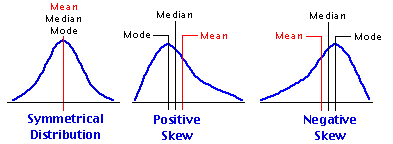
\includegraphics[width=0.7\textwidth]{img/skew.png}
        \caption{Skewness of distributions.}
    \end{figure}
    \item $\tilde{\mu}_4$ is called \textbf{kurtosis} and measures the dispersion of the random variable around the values $\mu+\sigma$ and $\mu - \sigma$. Specifically, the kurtosis of a distribution is compared to that of a Normal distribution, which is always 3. Then, if the kurtosis is equal to 3, the distribuion is \textbf{mesokurtic} (similar to a Normal); if it is greater than 3, it is \textbf{leptokurtic} (the tails are fatter, while the middle is thinner); if it is less than 3, it is \textbf{platykurtic} (the tails are thinner, but the middle is larger).
\end{itemize}\separate
\section{Distances between distributions}

\boxdefinition{Distances and metrics}{
    A distance over a set $\mathcal{A}$ is a function $d : \mathcal{A} \times \mathcal{A} \rightarrow \mathbb{R}$ such that:
    \begin{itemize}[itemsep=-1pt]
        \item $d(x,y) \geq 0$ (non-negativity)
        \item $d(x,y) = 0 \text{ iff } x=y$ (identity of indiscernibles)
        \item $d(x,y) = d(y,x)$ (symmetry)
    \end{itemize}
    Also, $d$ is a metric if it also satisfies the triangle inequality: $d(x,z) \leq d(x,y) + d(y,z)$.
}
Distances and metrics over probability distributions are used to measure how far apart two distributions are. Calculating distances is very useful in statistics and machine learning: for example, after a dataset has been split into training and test sets, we can compare the distribution of the two to make sure they are similar (or, alternatively, to make sure they are different and study how well the model generalizes). This section will overview the most common distances used in statistics.
\boxdefinition{Total Variation (TV) distance}{
    \vspace{-15pt}
    \begin{align*}
        &d_{TV}(X,Y) = \frac{1}{2} \sum_i |p_X(a_i) - p_y(a_i)| &\text{(discrete case)}\\
        &d_{TV}(X,Y) = \frac{1}{2} \int |f_X(x) - f_Y(x)| dx &\text{(continuous case)}
    \end{align*}
}
\boxdefinition{Kolmogorov-Smirnof (KS) distance}{
    \vspace{-15pt}    
    \begin{equation*}
        d_{KS}(X,Y) = \sup_x |F_X(x) - F_Y(x)| 
    \end{equation*}
}
Both are metrics. They have no closed forms, but they can be approximated from samples of the distributions.

\boxdefinition{Shannon's information entropy (H)}{
    \vspace{-15pt}
    \begin{align*}
        &H(X) = \E[-\log(p(X))] = -\sum_i p(a_i) \log(p(a_i)) &\text{(discrete case)} \\
        &H(X) = \E[-\log(f(X))] = -\int_{-\infty}^{\infty} f(x) \log(f(x)) dx &\text{(continuous case)}
    \end{align*}
}
Entropy measures the average level of information (or ``surprise'', ``uncertainty'') of a random variable. Information is inversely proportional to probability: the more unlikely an event is, the more information it carries. So, for example, a random variable that only takes a single value has zero entropy, because there is no uncertainty about its value. In contrast, a random variable that takes many values with equal probability has high entropy, because there is a lot of uncertainty about its value.

Let $X$ be a discrete random variable with a finite domain of $n$ elements. Per corollary of Jensen's inequality, since $log(x)$ is a concave function, we have:
\begin{equation*}
    H(X) = \E[-\log(p(X))] = \E\left [\log \left (\frac{1}{p(X)} \right ) \right ] \leq \log\left (\E \left [\frac{1}{p(X)} \right ] \right )
\end{equation*}
Then, by change of variable:
\begin{equation*}
    \E\left [ \frac{1}{p(X)} \right ] = \sum_i \frac{p(a_i)}{p(a_i)} = n
\end{equation*}
So we can derive the following bound for the entropy:
\begin{equation*}
    H(X) \leq \log(n)
\end{equation*}
\boxdefinition{Cross entropy (H)}{
    \vspace{-15pt}
    \begin{align*}
        &H(X;Y) = \E_X[- \log p_Y(Y)] = -\sum_i p_X(a_i) \log(p_Y(a_i)) &\text{(discrete case)} \\
        &H(X;Y) = \E_X[- \log f_Y(Y)] = -\int_{-\infty}^{\infty} f_X(x) \log(f_Y(x)) dx &\text{(continuous case)}
    \end{align*}
}
Cross entropy measures the number of bits needed to encode values from $X$ using a code based on $Y$. If the two have exactly the same distribution, the cross entropy is minimal: it is exactly equal to the entropy of $X$. The more the two are different, the more extra bits will be needed to encode the differences between the two.
\boxdefinition{Joint entropy (H)}{
    \vspace{-15pt}
    \begin{align*}
        &H(X,Y) = \E[-\log(p(X,Y))] = -\sum_{i,j} p(a_i,a_j) \log(p(a_i,a_j)) &\text{(discrete case)} \\
        &H(X,Y) = \E[-\log(f(X,Y))] = -\int_{-\infty}^{\infty} f(x,y) \log(f(x,y)) dx dy &\text{(continuous case)}
    \end{align*}
}
Joint entropy is simply the entropy of the joint distribution of two random variables $X$ and $Y$. If the two are independent, then $p_{XY}(x,y) = p_X(x) \cdot p_Y(y)$ (and similarly for PDFs), so the above sum/integral can be split, making it so that $H(X,Y) = H(X) + H(Y)$.
\boxdefinition{Kullback-Leibler (KL) divergence}{
    \vspace{-15pt}
    \begin{align*}
        &D_{KL}(X||Y) = \sum_i P_X(a_i) \log \left ( \frac{p_X(a_i)}{p_y(a_i)} \right ) = H(X;Y) - H(X) &\text{(discrete case)} \\
        &D_{KL}(X||Y) = \int_{-\infty}^{\infty} f_X(x) \log \left ( \frac{f_X(x)}{f_Y(x)} \right ) dx = H(X;Y) - H(X) &\text{(continuous case)}
    \end{align*}
}
KL divergence is also sometimes called relative entropy of $X$ w.r.t. $Y$; it measures how well the distribution of the model $Y$ can reconstruct the distribution of the data $X$. Since it can be expressed in terms of cross-entropy and entropy, it is easy to see that
\begin{itemize}[itemsep=0pt]
    \item It is always non-negative, since the cross-entropy between two distributions can only be greater than or equal to the entropy of one of them.
    \item It is exactly 0 if the two distributions are the same.
    \item It is asymmetric.
\end{itemize}
Note that since it is not symmetric, it is not an actual distance.
\boxdefinition{Mutual information}{
    \vspace{-18pt}
    \begin{align*}
        &\text{Discrete case:}\\
        &I(X,Y) = D_{KL}(p_{XY} || p_X p_Y) = \sum_{i,j} p_{XY}(a_i, a_j) \log \left ( \frac{p_{XY}(a_i, a_j)}{p_X(a_i)p_y(a_j)} \right ) = H(X) + H(Y) - H(X,Y)\\
        &\text{Continuous case:}\\
        &I(X,Y) = D_{KL}(f_{XY} || f_X f_Y) = \int_{-\infty}^{\infty} f_{XY}(x,y) \log \left ( \frac{f_{XY}(x,y)}{f_X(x)f_Y(y)} \right ) dx dy = H(X) + H(Y) - H(X,Y)
    \end{align*}
}
Mutual information measures how dependent the two distributions are. It quantifies how much the product of the marginals can reconstruct the joint distribution.
\begin{itemize}[itemsep=0pt]
    \item It is always non-negative, since the sum of the individual entropies is always greater than or equal to the joint entropy.
    \item It is exactly 0 if $X \indep Y$.
    \item It is symmetric.
\end{itemize}
In some cases, it may be useful to have a normalized measure of dependence. The \textbf{normalized mutual information} is defined as:
\begin{equation*}
    NMI(X,Y) = \frac{I(X,Y)}{\min\{H(X), H(Y)\}} \in [0,1]
\end{equation*}
Suppose we have an unknown variable $X$, and we observe a noisy function of it, called $Y$. Let $Z = f(Y)$, i.e., a processing of the noisy observations. Intuitively, $Z$ cannot contain more information about $X$ than $Y$ does. This is known as the \textbf{data processing inequality}:
\begin{equation*}
    I(X,Y) \geq I(X,Z)
\end{equation*}
If they happen to be equal, and $Z$ is a summary of $Y$, then $Z$ is a sufficient statistic for $X$: it means that we can reconstruct $X$ from $Z$ with the same accuracy as from $Y$.
\boxdefinition{Earth mover's distance (Wasserstein metric)}{
    \vspace{-15pt}
    \begin{align*}
        &EMD(X,Y) = \frac{\sum_{i,j} F_{i,j} \cdot |a_i - a_j|}{\sum_{i,j} F_{i,j}}
    \end{align*}
}
Earth's mover distance measures the minimum cost required to transform one distribution into another; the $F$ in the formulas is the \textbf{flow} which minimizes the numerator (the cost). In practice, for pairs of univariate random vairables $X$ and $Y$, is is calculated as follows:
\begin{align*}
    &EMD(X,Y) = \sum_i |F_X(a_i) - F_Y(a_i)| &\text{(discrete case)}\\
    &EMD(X,Y) = \int_{-\infty}^{\infty} |F_X(x) - F_Y(x)| \ dx &\text{(continuous case)}
\end{align*}
For empirical distributions, assuming the samples are sorted in increasing order:
\begin{equation*}
    EMD(X,Y) = \frac{1}{n} \sum_i |x_i - y_i|
\end{equation*}\separate
\section{The law of large numbers}

For many experiments that concern natural phenomena, different executions of the same experiment will likely yield different results. The variation in the outcome is due to randomness caused by uncontrollable factors. To mitigate the effect of this randomness, the same experiment can be repeated a number of times and the \textbf{average} of the results is studied instead. Formally, given $X_1, X_2, \dots, X_n$ independent random variables, their average is
\begin{equation*}
    \bar{X}_n = \frac{X_1 + X_2 + \ldots + X_n}{n}
\end{equation*}
\boxdefinition{Expected value and variance  of an average}{
    If $\bar{X}_n$ is the average of $n$ independent random variables with the same expectation $\mu$ and variance $\sigma^2$, then
    \begin{align*}
        &\E[\bar{X}_n] = \mu &Var(\bar{X}_n) = \frac{\sigma^2}{n}
    \end{align*}
}
The random variables do not need to be identically distributed. Note that the variance is inversely proportional to the number of random variables contributing to the average: the more variables we have, the more stable the average becomes.

\boxdefinition{Markov's inequality}{
    Let $X \geq 0$ be a random variable, and let $a > 0$. Then
    \begin{equation*}
        P(X \geq a) \leq \frac{\E[X]}{a}
    \end{equation*}
    \textbf{Corollary:} Assume $X \geq 0$, $\E[X] > 0$ and $k > 0$. Then
    \begin{equation*}
        P(X \geq k \E[X]) \leq \frac{1}{k}
    \end{equation*}
}
The proof is as follows: let $\mathbbm{1}_{X \geq \alpha}$ be an indicator variable that is 1 if $X \geq \alpha$ and 0 otherwise. Then
\begin{align*}
    \alpha \mathbbm{1}_{X \geq \alpha} \leq X\\
    \E[\alpha \mathbbm{1}_{X \geq \alpha}] \leq \E[X]\\
    \alpha P(X \geq \alpha) \leq \E[X]\\
    P(X \geq \alpha) \leq \frac{\E[X]}{\alpha}
\end{align*}

\boxdefinition{Chebyshev's inequality}{
    Let $X$ be a random variable, and $a > 0$. Then
    \begin{equation*}
        P(|X - \E[X]| \geq a) \leq \frac{Var(X)}{a^2} 
    \end{equation*}
}
This inequality claims that most of the probability mass of a random variable is within a few standard deviations from the expected value. It is a consequence of Markov's inequality:
\begin{align*}
    P(|X - \E[X]| \geq a) = P((X - \E[X])^2 \geq a^2) \leq \frac{\E[(X - \E[X])^2]}{a^2} = \frac{Var(X)}{a^2}
\end{align*}
Now, we can apply Chebyshev's inequality to the average of $n$ independent random variables, obtaining the following result:
\boxdefinition{The (weak) law of large numbers}{
    Let $\bar{X}_n$ be the average of $n$ independent random variables with the same expectation $\mu$ and variance $\sigma^2$. Then, for any $\varepsilon > 0$,
    \begin{equation*}
        \lim_{n \to \infty} P(|\bar{X}_n - \mu| > \varepsilon) = 0
    \end{equation*}
}
This law confirms what we previously observed with the variance of the average. As $n$ goes to infinity, the probability that the value of the average significantly deviates from its expectation (that is also the same of the individual random variables in the average) becomes zero. This also holds if $\sigma^2$ is infinite, as long as the individual random variables have finite expectation.

The consequence of the law of large numbers is that by calculating the average of a reasonably large enough set of random variables we can recover not only the mean and the stardard deviation, but pretty much any feature of the distribution of the random variables. Next up are two application examples.

\paragraph{Recovering the probability of an event} Assume we want to know the probability that the outcome of some experiment falls within a certain range, i.e., $p = P(a \leq X \leq b)$. We run $n$ independent measurements of this same experiment, and we model those results with the r.v.s $X_1, X_2, \dots, X_n$. Then, we can define an indicator variable for each $X_i$:
\begin{equation*}
    Y_i = \mathbbm{1}_{a \leq X_i \leq b} = \begin{cases}
        1 & \text{if } a \leq X_i \leq b\\
        0 & \text{otherwise}
    \end{cases}
\end{equation*}
The $Y_i$ are also independent (per the propagation of independence seen previously). Since $Y_i$ is an indicator variable, we know that
\begin{align*}
    &\E[Y_i] = p = P(a \leq X_i \leq b) &Var(Y_i) = p(1 - p)
\end{align*}
Let $\bar{Y}_n$ be the average of the indicator variables. By the law of large numbers:
\begin{equation*}
    \lim_{n \to \infty} P(|\bar{Y_n} - p| > \varepsilon) = 0
\end{equation*}
Informally, this means that if we perform the experiment $n$ times, count the amount of times the outcome falls within the range $[a, b]$, and divide by $n$, we get an estimate of the real probability of that event. The larger $n$ is, the better the estimate becomes.

\paragraph{Estimating conditional probability} We want to estimate the conditional probability for two random variables: $p = P(C = c | A = a) = P(A=a, C=c)/P(A=a) = p_{ac}/p_a$. We run $n$ independent measurements of the experiment, modeling each result as a pair $(A_i, C_i)$. We define indicator variables as the example above:
\begin{align*}
    &Y_i = \mathbbm{1}_{A_i = a \land C_i = c} = \begin{cases}
        1 & \text{if } A_i = a \land C_i = c\\
        0 & \text{otherwise}
    \end{cases}\\
    &Z_i = \mathbbm{1}_{A_i = a} = \begin{cases}
        1 & \text{if } A_i = a\\
        0 & \text{otherwise}
    \end{cases}
\end{align*}
By applying the (strong) law of large numbers, we get that
\begin{align*}
    \lim_{n \to \infty} P(\bar{Y}_n = p_{ac}) = 1 \\
    \lim_{n \to \infty} P(\bar{Z}_n = p_a) = 1
\end{align*}
The two limits can be condensed in a ratio to estimate the conditional probability:
\begin{equation*}
    \lim_{n \to \infty} P(\frac{\bar{Y}_n}{\bar{Z}_n} = \frac{p_{ac}}{p_a}) = 1
\end{equation*}

\boxdefinition{Hoeffding bound}{
    If $\bar{X}_n$ is the average of $n$ independent random variables with the same expectation $\mu$ and $P(a \leq X_i \leq b) = 1$, then for any $\varepsilon > 0$:
    \begin{equation*}
        P(|\bar{X}_n - \mu| \geq \varepsilon) \leq 2e^{-2n\varepsilon^2 / (b-a)^2} 
    \end{equation*}
}
This offers a tight bound on the probability that the average deviates from its expectation by an arbitrarily small amount, but requires that the random variables have a bounded support.

\section{The central limit theorem}

\boxdefinition{The central limit theorem}{
    Let $X_1, X_2, \dots, X_n$ ne any sequence of i.i.d. random variables with the same expectation $\mu$ and finite positive vairance $\sigma^2$. For $n \geq 1$, let $Z_n$ be defined by
    \begin{equation*}
        Z_n = \sqrt{n}\frac{\bar{X}_n - \mu}{\sigma}
    \end{equation*}
    Then, for any number $a$
    \begin{equation*}
        \lim_{n \to \infty} F_{Z_n} (a) = \Phi(a)
    \end{equation*}
    where $\Phi$ is the distribution function of the $\mathcal{N}(0,1)$ distribution.
}
This theorem states that if we take the average of $n$ random variables, remove its expectation, and divide by its standard deviation, the result is a random variable that converges to a standard normal distribution as $n$ goes to infinity. But, in practice, how large should $n$ be? A famous rule of thumb is to use $n \geq 30$ to get a good approximation, but it is mostly just a myth; the optimal value of $n$ depends on the distribution of the random variables.

\separate
\section{Summaries}

Summaries are used to represent and describe the information contained in datasets. They csan be graphical summaries, which visually represent the data, or numerical summaries, which give a description of the data in terms of numbers.

\subsection{Graphical summaries}
\paragraph{Empirical CDF} A random variable is completely characterized by its CDF. We can approximate the CDF with the empirical cumulative distribution function, which is defined as
\begin{equation*}
    F_n(x) = \frac{|\{ i : [1,n] | x_i \leq x \}|}{n}
\end{equation*}
where the $x_i$ are the observations in the dataset. The \textbf{Glivenko-Cantelli theorem} states that the empirical CDF converges to the true CDF as $n$ goes to infinity:
\begin{equation*}
    P(\lim_{n \to \infty} \sup_x |F(x) - F_n(x)| = 0) = 1
\end{equation*}
This approximation can be plugged into different formulas to estimate other quantities, such as the mean or the variance.

\paragraph{Bar plots and histograms}
A bar plot is used for discrete data. It provides a frequency count for the values in the dataset, and approximates the PMF (as a consequence of the law of large numbers, as seen in a previous example):
\begin{equation*}
    P(X = a) \approx \frac{|\{ i | x_i = a \}|}{n}
\end{equation*}
A histogram is used for continuous data. It provides frequency counts for ranges of values (instead of individual ones). The support of the random variable is first split into $m$ intervals called \textbf{bins} (which can all have the same width or different widths), and the number of occurrences belonging to each bin is counted and normalized:
\begin{equation*}
    A_i = \frac{|\{ j \in [1,n] |x_j \in B_j\}|}{n} \approx P(X \in B_i)
\end{equation*}
The bins can be plotted as rectangles so that their area is proportional to $A_i$; after fixing their width $b_i$, the height is found as $H_i = A_i / b_i$.

Bin width can be chosen in different ways, producing different results. It is common to choose the same width for all bins, such that, for a total number of bins $m$, the interval corresponding to the $i^{th}$ bin is
\begin{equation*}
    B_i = (r + (i-1)b, r + i*b)
\end{equation*}
where $r$ is the minimum value taken by the random variable, and $b$ is the bin width. The optimal width can be found using \textbf{Mean Integrated Squared Error} (\textbf{MISE}):
\begin{equation*}
    MISE = \E \left [ \int (\hat{f}(t) - f(t))^2 \ dt \right ] = \int \int (\hat{f}(t) - f(t))^2 f(x_1) \ldots f(x_n) \ dt dx_1 \ldots dx_n
\end{equation*}
where $\hat{f}$ is the density estimation of the real PDF $f$. The minimum of the MISE for Normal distributions is represented by \textbf{Scott's normal reference rule}:
\begin{equation*}
    b = 3.49 \cdot s \cdot n^{-1/3}
\end{equation*}
wher $s$ is the sample standard deviation.\\
Other options are:
\begin{itemize}
    \item \textbf{Freedman-Diaconis' choice}:
    \begin{equation*}
        b = 2 \cdot \text{IQR} \cdot n^{-1/3}
    \end{equation*}
    This choice is more robust to outliers than the previous.
    \item \textbf{Variable bin width} (such as logarithmic binning as seen in power-law distributions).
    \item \textbf{Fixing the number of bins, and derivaring the width from it}. Some common strategies are:
    \begin{align*}
        &m = \lceil \frac{\max x_i - \min x_i}{b} \rceil\\
        &m = \lceil \sqrt{n} \rceil\\
        &m = \lceil \log_2 n \rceil + 1 \text{ (Sturges' rule)}
    \end{align*}
    The latter assumes normal distribution for the true density. This distribution can be approximated by a $Bin(n, 0.5)$ distribution, so the absolute frequency of the $i^{th}$ bin is $\binom{m-1}{i}$. The total frequency is $n = \sum_{i=0}^{m-1} \binom{m-1}{i} = 2^{m-1}$, from which $m$ is derived.
\end{itemize}

\paragraph{Kernel density estimation}
A big disadvantage of histograms is that the result strictly depends on the number of bins/bin width chosen to visualize the data. Kernel density estimation is another popular method to summarize distributions which is not as sensitive to the choice of parameters.

The idea behind this method is to mix kernel functions (which can take different forms, see Fig \ref{fig:kernels}) centered in each observation in the dataset. Since data is assumed to be of continuous nature, the presence of a certain value in the dataset also contributes to the density of the values around it. The kernel function models the way this density is distributed around that single observation, and by mixing together all the kernels, the result should be a good approximation of the true density.
\begin{figure}[h]
    \centering
    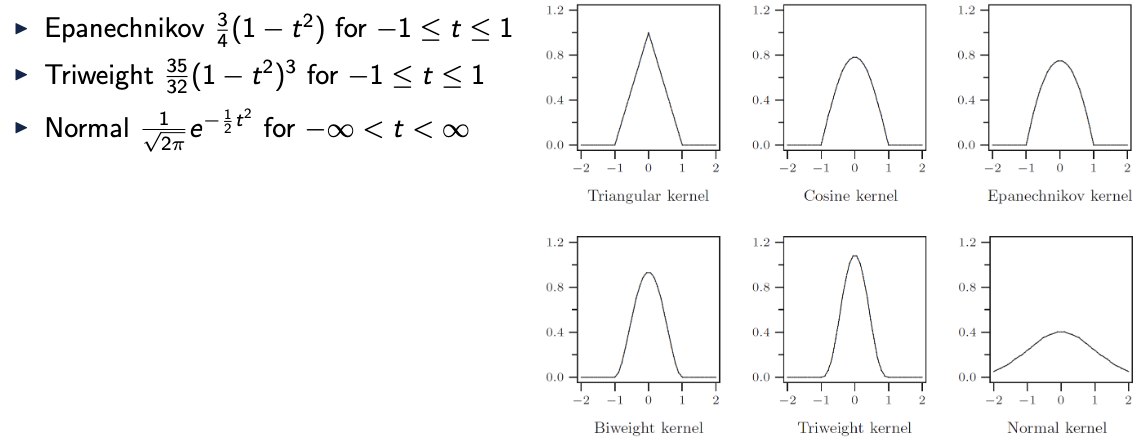
\includegraphics[width=0.8\textwidth]{img/kernels.png}
    \caption{Examples of common kernels used in KDE.}
    \label{fig:kernels}
\end{figure} \\
\boxdefinition{Kernel}{
    A kernel is a function $K : \mathbb{R} \to \mathbb{R}$ such that
    \begin{itemize}
        \item $K$ is a probability density: $K(t) \geq 0$ and $\int_{-\infty}^{\infty} K(t) \ dt = 1$
        \item $K$ is symmetric: $K(-t) = K(t)$
        \item $K(t) = 0$ for $|t| > 1$ (i.e., support is $[-1, 1]$)
    \end{itemize}
}
The last requirement is not strictly necessary, actually; for example, the Normal kernel has unbounded support.

Each kernel function is characterized by a center (the observation), and a \textbf{bandwidth} $h$, which is a scaling factor over the support of the kernel from $[-1, 1]$ to $[-h, h]$. In other words, the badwidth determines how tall-thin or short-wide the kernel is around its center. We can then write
\[
    X \sim K(t) \implies h \cdot X + x_i \sim \frac{1}{h} K \left ( \frac{t - x_i}{h} \right )
\]
because of the change-of-units transformation formulas. The final kernel density estimate is the result of the \textbf{mixture} of all the scaled and shifted kernel densities:
\begin{equation*}
    f_{n,h} (t) = \frac{1}{nh} \sum_{i=1}^n K\left ( \frac{t-x_i}{h}\right )
\end{equation*}
The $1/n$ in the formula is a normalization factor that ensures the density integrates to 1.

The choice of kernel is not critical to the final result; different kernels behave similarly. The key parameter is the bandwidth $h$. Also for KDE, MISE can be used to find the optimal value. Assuming the true density is Normal, the MISE is minimized for
\begin{equation*}
    h = \left (\frac{4}{3} \right )^{1/5} \cdot s \cdot n^{-1/5}
\end{equation*}
For other distributions, the optimal bandwidth can be found using plug-in selectors or cross validation selectors.

Another issue that may arise is when the support of the random variable is bounded. If KDE is used as is, the result will present density event corresponding to values that are not possible. To avoid this, boundary correction techniques are used; some examples are
\begin{itemize}
    \item Kernel truncation and renormalization (forced truncation of the kernel outside the support);
    \item Linear combination kernel;
    \item Beta boundary kernels;
    \item Reflective kernels.
\end{itemize}

\subsection{Numerical summaries}

\paragraph{Sample summaries} Summaries of the empirical data can be used to estimate summaries of the true distribution. The following are some common ones:
\begin{itemize}
    \item \textbf{Sample mean}:
    \begin{equation*}
        \bar{x} = \frac{x_1 + \ldots + x_n}{n}
    \end{equation*}
    \item \textbf{Median}:
    Let $x_1, x_2, \ldots, x_n$ be the data in the sample, sorted.
    \begin{equation*}
        Med(x_1, \ldots, x_n) = \begin{cases}
            x_{n/2} &\text{if } n \text{ is odd}\\
            \frac{x_{n/2} + x_{n/2 + 1}}{2} &\text{if } n \text{ is even} 
        \end{cases}
    \end{equation*}
    The median of a distriution corresponds to the $0.5^{th}$ quantile.
    \item \textbf{Sample variance and standard deviation}:
    \begin{align*}
        &s_n^2 = \frac{\sum_i^n (x_i - \bar{x_n})^2}{n-1} & s_n = \sqrt{s_n^2}
    \end{align*}
    \item \textbf{Median of absolute deviations}:
    \begin{equation*}
        MAD(x_1, \ldots, x_n) = Med(|x_1 - Med(x_1, \ldots, x_n)|, \ldots, |x_n - Med(x_1, \ldots, x_n|))
    \end{equation*}
    If the distribution is symmetric, the MAD is exactly equal to the difference between the $0.75^{th}$ and $0.5^{th}$ quantiles.
\end{itemize}

\paragraph{Order statistics} Let $x_1, x_2, \ldots, x_n$ be the ordered sequence of values in a sample. $x_{\langle i \rangle}$ is the $i^{th}$ order statistic. Order statistics are used to calculate empirical quantiles. Formally, the $p^{th}$ quantile is the value $q_p$ such that $q_p = \inf_x \{ P(X \leq x) \geq p \} = \inf_x \{F(x) \geq p\}$ (to be read as: ``the smallest number $x$ such that the probability of $X$ being less or equal than $x$ is greater or equal than $p$''). To find the empirical quantiles, we use the empirical approximation of the CDF in place of the true CDF:
\[
    q_p = \inf_x \{ F_n(x) \geq p \} = \inf_x \left\{\frac{|\{i | x_i \leq x \}|}{n} \geq p \right\}
\]
There are actually many ways to find the quantiles of a distribution. In \texttt{R}, there are 9 variants. The default one is type 7:
\begin{equation*}
    p = \frac{i-1}{n-1} \implies q_p = x_{\langle p\cdot(n-1) + 1 \rangle}
\end{equation*}
Another common choice is type 6:
\begin{equation*}
    p = \frac{i}{n+1} \implies q_p = x_{\langle p \cdot (n+1) \rangle}
\end{equation*}
The difference between the methods is irrelevant for big enough datasets.

What if the supposed index of the quantile is not an integer? In this case, the quantile is approximated using linear interpolation. Let $k = \lfloor p \cdot (n+1) \rfloor$ (or whatever other formula is used by the chosen method). Then,
\begin{equation*}
    q_p = x_{\langle k \rangle} + \alpha \cdot (x_{\langle k+1 \rangle} - x_{\langle k \rangle})
\end{equation*}
where $\alpha = p \cdot (n+1) - k$, i.e., the decimal part of the index.

\paragraph{Association and correlation}
\textbf{Association} measures how much information one variable provides on another. If two variables are independent, they are not associated. Association is maximum when one variable is a (invertible) function of the other. \textbf{Correlation} measures the presence and strenght of an increasing/decreasing trend between two variables. If two variables are independent, their correlation is always 0, but the opposite is not always true.
\boxdefinition{Correlation}{
    Let $X$ and $Y$ be two random variables. The correlation coefficient $\rho$ is defined to be 0 if $Var(X) = 0$ or $Var(Y) = 0$, and otherwise as
    \begin{eqnarray}
        \rho = \frac{Cov(X, Y)}{\sqrt{Var(X) \cdot Var(Y)}}
    \end{eqnarray}
}
Some common correlation coefficients are:
\begin{itemize}
    \item \textbf{Pearson's r}: it is obtained by substituting the sample covariance and the sample standard deviations of the random variables in the formula above:
    \begin{align*}
        &s_{xy} = \frac{\sum_{i=1}^n (x_i - \bar{x}) \cdot (y_i - \bar{y})}{n-1} &r = \frac{s_{xy}}{s_x \cdot s_y}
    \end{align*}
    It is bounded in the interval $[-1,1]$. The computational cost to calculate it is $O(n)$. A limitation of Pearson's r is that it can only detect linear relationships between random variables, and it can only be used when the variables are continuous.
    \item \textbf{Spearman's $\rho$}: this coefficient is calculated as the correlation between ranks of the observations. Let $\textit{rank}(x)$ be the ranks of the values of the variable $x$. Then, Spearman's $\rho$ is calculated as
    \begin{equation*}
        \rho = r(\textit{rank}(x), \textit{rank}(y)) = 1 - \frac{6 \sum_{i=1}^n (rank(x)_i - rank(y)_i)^2}{n\cdot(n^2 - 1)} 
    \end{equation*}
    This coefficient assesses monotonic relationships of any kind (both linear and non-linear). The computational cost to calculate it is $O(n \cdot \log n)$, since it requires a sorting of the data to compute the ranks. It can be used when both variables are ordinal, continuous, or when one is ordinal and the other is continuous.
    \item \textbf{Kendall's $\tau$}: this coefficient compares the sign of the differences between successive pairs of observations. It is calculated as
    \begin{equation*}
        \tau_a = \frac{2 \sum_{i<j} \textit{sign}(x_i - x_j) \cdot \textit{sign}(y_i - y_j)}{n \cdot (n-1)}
    \end{equation*}
    It calculates the fraction of concordant pairs minus discordant pairs of values between the two variables, and it is bounded in the interval $[-1,1]$. The computational cost to calculate it is $O(n^2)$. There is a variant, $\tau_b$, which also takes into account the possibility of ties; instead of dividing by $n \cdot (n-1)$, it counts how many pairs do not present a tie in $x$ or $y$. It can be used when both variables are ordinal, or when one is ordinal and the other is continuous.
    \item \textbf{Somer's D}: this coefficient is used when one variable is continuous and the other is binary. It can be seen as an asymmetric version of Kendall's $\tau$:
    \begin{eqnarray}
        D = \frac{\tau_{xy}}{\tau{yy}} = \frac{\sum_{i<j} \textit{sign}(x_i - x_j) \cdot \textit{sign}(y_i - y_j)}{\sum_{i<j} \textit{sign}(y_i - y_j)^2}
    \end{eqnarray}
    It calculates the fraction of concordant pairs minus discordant pairs over the number of unequal pairs of values in $y$. An example application can be seen with probabilistic classifiers: $x$ is the confidence prediction of an example being positive, $y$ is the true class, and $D$ is the Gini index of the classifier.
    \item \textbf{Thiel's U}: it is used when both variables are nominal. It can be calculated in a symmetric and an asymmetric way:
    \begin{align*}
        &U_{sym} = \frac{2 \cdot I(X,Y)}{H(X) + H(Y)} &U_{asym} = \frac{I(X,Y)}{H(X)}
    \end{align*}
    where $I(X,Y)$ is the mutual information between $X$ and $Y$, and $H(X), H(Y)$ are the entropies of the two random variables. The asymmetrical version, specifically, indicates what fraction of $X$ can be predicted by $Y$.
\end{itemize}\separate
\section{Estimators}

A dataset is a st of repeated measurements of a specific phenomenon which we want to understand better. The phenomenon can be modeled using some probability distribuion, so the dataset (which is the realization of a random sample from that distribution) can be used to approximate its parameters.
\boxdefinition{Random sample}{
    A random sample is a collection of i.i.d. random variables $X_1, X_2, \ldots, X_n \sim F(\alpha)$, where $F()$ is the distribution and $\alpha$ its parameter(s).
}
A classic example is the approximation of the speed of light by physicist A. A. Michelson, done in 1879. His dataset of measurements consisted of 100 different measurements, each which was in itself th average of repeated measurements on several variables (e.g., distance between the tools used). At the end, his estimate was off by about 150 km/s, likely due to him missing some source of error despite his meticulousness; still, he had the intuition of using the average of a dataset to estimate the parameter of a distribution (in this case, the one that describes the speed of light).
\boxdefinition{Estimand and estimate}{
    An estimand $\theta$ is an unknown parameter of a distribution $F()$. \\
    An estimate $t$ of $\theta$ is a value that is obtained as a function $h()$ over a dataset:
    \begin{eqnarray}
        t = h(x_1, \ldots, x_n)
    \end{eqnarray}
}
\boxdefinition{Statistics and estimator}{
    A statistics is a function $h(X_1, \ldots, X_n)$ of random variables. \\
    An estimator of a parameter $\theta$ is a statistics $T_n = h(X_1, \ldots, X_n)$ intended to provide information about $\theta$.
}
Using the speed of light example, we can model is as follows: the dataset of measurements is the realization of a random sample of random variables. Each random variable is defined as:
\begin{equation*}
    X_i = c + \epsilon_i
\end{equation*}   
where $c$ is the speed of light, and $\epsilon_i$ is a measurement error, assumed to be normally distributed with mean 0 ad variance $\sigma^2$. The \textbf{estimand} is the expected value of one of these variables: $\theta = \E[X_i]$. We can define an \textbf{estimator} as the average of the sample:
\begin{equation*}
    T_n = \bar{X}_n = \sum_{i=1}^n \frac{X_1 + X_2, \ldots, + X_n}{n}
\end{equation*}   
Finally, the \textbf{estimate} is the actual value we get by plugging the values collected in the dataset to the estimator.

\boxdefinition{Unbiased estimator}{
    An estimator $T_n = h(X_1, \ldots, X_n)$ of a parameter $\theta$ is unbiased if
    \begin{equation*}
        \E[T_n] = \theta
    \end{equation*}
    If $\E[T_n] - \theta \not = 0$, the estimator is biased.
}
Bias, if present, can be either positive or negative. An estimator may be \textbf{asymptotically unbiased} if it its unbiased as the sample size $n$ approaches infinity:
\begin{equation*}
    \lim_{n \to \infty} \E[T_n] = \theta
\end{equation*}
Sometimes, the estimator is indicated with the same symbol as the estimand, but with a hat on top: $\hat{\theta}$ (e.g., $\hat{\mu}$ is an estimator for the mean, $\hat{sigma}$ is an estimator for the standard deviation).

Bias can be thought of as a measure of how well the estimator can approsimate the parameter of interest. If it is unbiased, it means it has the capacity to estimate the parameter correctly. Estimators are also characterized by their variance. \textbf{Variance} is a measure of how much the estimate can sway from the true value of the parameter, regardless of bias. An estimator can have low bias, but high variance, meaning that it can approximate the parameter, but the response is not necessarily reliable. When the same estimand has multiple unbiased estimators, variance is a measure of their efficiency. Let $T_1$ and $T_2$ be unbiased estimators of $\theta$; $T_1$ is \textbf{more efficient} than $T_1$ if $Var(T_2) < Var(T_1)$. The \textbf{relative efficiency} of $T_2$ w.r.t. $T_1$ is $Var(T_1)/Var(T_2)$. The standard deviation of the estimator is called \textbf{standard error} (\textbf{SE}).
\boxdefinition{Unbiased estimators for expectation and variance}{
    Let $X_1, X_2, \ldots, X_n$ be a random sample from a distribution with finite expectation $\mu$ and finite variance $\sigma$. Then
    \begin{equation*}
    \bar{X}_n = \frac{X_1 + X_2 + \ldots + X_n}{n}
\end{equation*}   
    is an unbiased estimator for $\mu$, and
    \begin{equation*}
    S^2 = \frac{1}{n-1} \sum_{i=1}^n (X_i - \bar{X}_n)^2
\end{equation*}   
    is an unbiased estimator for $\sigma^2$.
}
We've already seen how the expected value of the mean is also the mean of the distribution. Also, per the central limit theorem, the variance of the mean goes to 0 as $n$ goes to infinity.

Why is the estimator of the variance divided by $n-1$ instead of $n$? This is called Bessel's correction, and it is used to make sure the estimator is unbiased. The proof is explained below. First, for any random variable $X_i$, the following hold true:
\begin{align*}
    &(1)\quad \E[X_i - \bar{X}_n] = \E[X_i] - \E[\bar{X}_n] = \mu - \mu = 0 \\
    &(2)\quad Var(X_i - \bar{X}_n) = \E[(X_i - \bar{X}_n)^2] - E[X_i - \bar{X}_n]^2 = \E[(X_i - \bar{X}_n)^2] = \sigma^2
\end{align*}
$X_i$ and $\bar{X}_n$ are not independent, because the latter is a function of the former. However, we can split the mean, removing $X_i$ from it, getting two independent terms:
\begin{equation*}
    X_i - \bar{X}_n = X_i - \frac{1}{n} \sum_{j=1}^n X_j = X_i - \frac{1}{n} X_i - \frac{1}{n} \sum_{j=1, j \not = i} X_j = \frac{n - 1}{n} X_i - \frac{1}{n} \sum_{j=1, j \not = i} X_j
\end{equation*}   
We can now easily calculate the variance, since it is the sum of the variances of the two terms:
\begin{gather*}
    Var(X_i - \bar{X}_n) = Var\left(\frac{n - 1}{n} X_i - \frac{1}{n} \sum_{j=1, j \not = i} X_j\right) = Var\left(\frac{n - 1}{n} X_i\right) + Var\left(\frac{1}{n} \sum_{j=1, j \not = i} X_j\right) =\\
    = \frac{(n - 1)^2}{n^2} \sigma^2 - \frac{1}{n^2} (n-1) \sigma^2 = \frac{n-1}{n} \sigma^2
\end{gather*}
Finally, we apply the above calculations to find the expected value of the estimator for the variance:
\begin{gather*}
    \E[S_n^2] = \E\left[\frac{1}{n-1} \sum_{i=1}^n (X_i - \bar{X}_n)^2\right] = \frac{1}{n-1} \sum_{i=1}^n \E[(X_i - \bar{X}_n)^2] =\\
    = \frac{1}{n-1} \sum_{i=1}^n Var(X_i - \bar{X}_n) = \frac{1}{n-1} n \frac{n-1}{n} \sigma^2 = \sigma^2
\end{gather*}
Additionally,
\begin{equation*}
    Var(S_n)^2 = \frac{1}{n}(\mu_4 - \frac{n-3}{n-1}\sigma^4)
\end{equation*}   
which goes to 0 as $n$ goes to infinity.\\
Intuitively, the need for this correction can be explained by the fact that the $X_i$ and the mean $\bar{X}_n$ are not independent; if we know $n-1$ random variables and the mean, we can always deduce the $n^{th}$ random variable. In this sense, the estimator has $n-1$ \textbf{degrees of freedom}: in general, the degrees of freedom of any estimator is the number of observations minus the number of parameters already estimated.

What about the standard deviation? Unfortunately, the square root of the estimator of the variance is not an unbiased estimator for the standard deviation. By Jensen's inequality, since the square root is a concave function, we have:
\begin{equation*}
    \E[\sqrt{S_n^2}] = \E[S_n] < \sqrt{\E[S_n^2]} = \sigma 
\end{equation*}   
This is true for most estimators: if $T$ is unbiased for $\theta$, $g(T)$ is not necessarily unbiased for $g(\theta)$; the only exception is when $g()$ is a linear transformation (since by Jensen's inequality the strict equality holds). A non-parametric unbiased estimator for the standard deviation does not exist: we need to know the distribution to estimate it unbiasedly.

\boxdefinition{Unbiased estimator for the median}{
    Let $X_1, \ldots, X_n$ be a random sample from a distribution with PDF $f(x)$. Let $m = F^{-1}(0.5)$ be the true median of the distribution. Let
    \begin{equation*}
        T = Med(X_1, \ldots, X_n).
\end{equation*}   
    Then
    \begin{equation*}
        T \sim N\left(m, \frac{1}{4n f(m)^2}\right) \quad \text{as} \quad n \to \infty
\end{equation*}   
    and $T$ is an unbiased estimator for the median as $n$ goes to infinity.
}
\boxdefinition{Unbiased estimator for quantiles}{
    Let $X_1, \ldots, X_n$ be a random sample from a distribution with PDF $f(x)$. Let $q_p$ the the true $p^{th}$ quantile of the distribution. Let
    \begin{equation*}
        T = q_{X_1, \ldots, X_n}(p)
\end{equation*}   
    Then
    \begin{equation*}
        T \sim N\left(q_p, \frac{p(1-p)}{n f(q_p)^2}\right) \quad \text{as} \quad n \to \infty
\end{equation*}   
    and $T$ is an unbiased estimator for the $p^{th}$ quantile as $n$ goes to infinity.
}
\boxdefinition{Unbiased estimator for the Median of Absolute Deviations (MAD)}{
    Let $X_1, \ldots, X_n$ be a random sample from a distribution. Let $Md$ be the true median of absolute deviations of the distribution. Let
    \begin{equation*}
        T = MAD(X_1, \ldots, X_n) = Med(|X_1 - Med(X_1, \ldots, X_n)|, \ldots, |X_n - Med(X_1, \ldots, X_n)|)
    \end{equation*}   
    Then
    \begin{equation*}
        T \sim N\left( Md, \frac{\sigma_1^2}{n} \right)
    \end{equation*}   
    (where $\sigma_1^2$ is defined in terms of $Md$, median, and CDF of the distribution) and $T$ is an unbiased estimator for the MAD as $n$ goes to infinity.  
}
All the above estimators are found by applying the corresponding version of the central limit theorem (CLT for medians, CLT for quantiles, CLT for MAD).

For correlation, the various coefficients seen in the previous section are estimators of the true correlation coefficient between two random variables. Pearson's $r$ is an estimator for $\rho$, but the distribution of $r$ is highly skewed. To fix this issue, the \textbf{Fisher transformation} can be applied, defined as follows: $\textit{FisherZ}(r) = \frac{1}{2} \log\frac{1+r}{1-r}$. The distribution of the Fisher-transformed coefficient is approximately normal:
\begin{equation*}
    \textit{FisherZ}(r) \sim N\left(\textit{FisherZ}(\rho), \frac{1}{n-3}\right)
\end{equation*}   
Hence, if we apply the inverse transformation to its expected value we get
\begin{equation*}
    \textit{FisherZ}^{-1} (\E[\textit{FisherZ(r)}]) = \rho
\end{equation*}   
This is also true for Spearman's $\rho$, sicne it is a special case of Pearson's $r$. \\
For Kendall's $\tau_a$, we have, for $n > 10$, that
\begin{equation*}
    \tau_a (X,Y) \sim N\left(\theta, \frac{2(2n + 5)}{9n(n-1)}\right)
\end{equation*}   
where $\theta = \E_{X_1,X_2 \sim F_X, Y_1, Y_2 \sim F_Y}[sign(X_1 - X_2) \cdot \textit{sign}(Y_1 - Y_2)]$. Hence $\tau_a$ is an unbiased estimator for $\theta$.
\boxdefinition{Mean Squared Error (MSE)}{
    The Mean Squared Error of an estimator $T$ for a parameter $\theta$ is defined as
    \begin{equation*}
        MSE(T) = \E[(T - \theta)^2]
\end{equation*}   
}
The MSE can be used to compare different estimators by considering both their bias and variance. The lower the MSE, the better the estimator. The MSE can be decomposed into the sum of the variance and the square of the bias:
\begin{gather*}
    MSE(T) = \E[(T - \E[T] + \E[T] - \theta)^2] =\\
    = \E[(T - \E[T])^2] + (\E[T] - \theta)^2 + 2\underset{(\textit{this is 0})}{\underbrace{{\E[T - \E[T]]}}}(E[T]- \theta) = \textit{Var}(T) + \textit{Bias}(T)^2
\end{gather*}
A biased estimator with low variance may be better than an unbiased estimator with high variance, since the latter may have a higher MSE.

\boxdefinition{Consistent estimator}{
    An estimator $T_n$ is a squared error consistent estimator if 
    \begin{equation*}
        \lim_{n \to \infty} MSE(T_n) = 0
\end{equation*}   
}
A consistent estimator has both bias and variance go to 0 as $n$ goes to 0. For example, $\bar{X}_n$ is a squared error consistent estimator of $\mu$.
\boxdefinition{Minimum Variance Unbiased Estimator (MVUE)}{
    An unbiased estimator $T_n$ of $\theta$ is a Minimum Variance Unbiased Estimator if
    \begin{equation*}
        Var(T_n) \leq Var(S_n)
\end{equation*}   
    for all unbiased estimators $S_n$ of $\theta$.
}
As a corollary, if $T_n$ is a MVUE, then $MSE(T_n) \leq MSE(S_n)$. $\bar{X}_n$ is also a MVUE of $\mu$ when the random sample is normally distributed with parameters $\mu$ and $\sigma^2$.\separate
\section{Maximum Likelihood Estimation}

The previous sections showed different ways to derive parameter estimators using the ``plug-in method'': knowing a sample, we use a formula of random variables, substitute the empirical data, and obtain an estimate. This section will introduce a more general parametric principle to derive estimators, called \textbf{Maximum Likelihood Estimation} (\textbf{MLE}). The maximum likelihood principle states: ``Given a dataset, choose the parameter(s) of interest that maximize the likelihood of observing that dataset''. 

\boxdefinition{Likelihood, Log-likelihood}{
    Let $x_1, \ldots, x_n$ be a dataset, realization of a random sample $X_1, \ldots, X_n$, where the PMF/PDF of $X_i$ is $f_{\theta}()$, parametric on $\theta$. The likelihood function is defined as
    \begin{equation*}
        L(\theta) = \prod_{i=1}^n f_{\theta}(x_i)
\end{equation*}   
    and the log likelihood function is defined as
    \begin{equation*}
        l(\theta) = \log L(\theta) = \sum_{i=1}^n \log f_{\theta}(x_i)
\end{equation*}   
}
The goal of MLE is to find the parameter value(s) that maximize the likelihood of the data. Since finding the maximum (in practice, derivating) a product is difficult, the logarithm of it is used instead, since it is a monotonic function (so the maximum remains the same) and the original likelihood can be converted to a sum of terms. Another issue to consider when using products is that when it is computed, the result can become very small, leading to numerical instability.
\boxdefinition{Maximum Likelihood estimates}{
    The maximum likelihood estimates of $\theta$ is the value $t = \arg\max_{\theta} L(\theta) = \arg\max_{\theta} l(\theta)$. The statistics over the random sample
    \begin{equation*}
        \hat{\theta}_{ML} = \arg\max_{\theta} L(\theta) = \arg\max_{\theta} l(\theta)
\end{equation*}   
    is called maximum likelihood estimator for $\theta$.
}
Often, loss functions are used to evaluate the quality of the estimator. Some examples are:
\begin{itemize}
    \item \textbf{Negative log-likelihood}: $nLL(\theta) = -l(\theta)$
    \item \textbf{Akaike Information Criterion} (\textbf{AIC}): $AIC = 2 |\theta| - 2 l(\theta)$. This function balances model fit (in the second term) with model simplicity (in the first term).
    \item \textbf{Bayesian Information Criterion} (\textbf{BIC}): $BIC = |\theta| \log(\theta) - 2 l(\theta)$. It has a stronger penalty for model complexity compared to AIC.
\end{itemize}
The last two can be used to compare models with different number of parameters since they consider complexity as well as fit.

MLE estimators can be biased, but under mild assumptions, they are always asymtotically unbiased, and (also asymptotically) they always have the smallest variance among unbiased estimators. Additionally, if $\hat{\theta}$ is the MLE estimator of $\theta$ and $g()$ is an invertible function, $g(\hat{\theta})$ is the MLE estimator of $g(\theta)$.

\paragraph{Cross entropy and negative log likelihood} There is a connection between the cross entropy and the negative log likelihood functions. Assume we have the random variables $X,Y$ with PMF $p_x$ and $p_y$. The cross entropy of $X$ with respect to $Y$ is defined as
\begin{equation*}
    H(X;Y) = - \sum_i p_x(a_i) \log p_y(a_i).
\end{equation*}   
The negative log-likelihood is
\begin{equation*}
    nLL(\theta) = - \sum_i \underset{\textit{This is } \log p_y(a_i)}{\underbrace{\log(f_{\theta}(x_i))}} = H(X;Y)
\end{equation*}   
where $X \sim F_n$ and $Y \sim F_{\theta}$. Minimizing the cross entropy (or the KL-divergence) between empirical and theoretical distributions is equivalent to maximizing the likelihood of the data.

\paragraph{Score function and Fisher Information}
The entropy of a random variable is the mean information carried by it. Then, the partial derivative (w.r.t. $\theta$) of the logarithm of $f_{\theta}$ represents the change in information as $\theta$ varies. It turns out that
\begin{equation*}
    \E\left[\frac{\partial}{\partial \theta} \log f_{\theta}(X)\right] = 0
\end{equation*}   
for any $X$. Instead of studying the expectation, we consider the variance. Formally, we define the score function and the Fisher information as follows:
\boxdefinition{Score function}{
    The score function is the random variable
    \begin{equation*}
        S(\theta) = \frac{\partial}{\partial \theta} l(\theta) = \sum_{i=1}^n \frac{\partial}{\partial \theta} \log f_{\theta}(X_i)
\end{equation*}   
}
\boxdefinition{Fisher information}{
    The Fisher information is the variance of th score function:
    \begin{equation*}
        I(\theta) = Var(S(\theta)) = \E[S(\theta^2)]
\end{equation*}   
}
The Fisher information measures the sensitivity of $X$ with respect to $\theta$. If small changes in $\theta$ cause large changes in the density function, the Fisher information is high: this means that the data provides information on the correct $\theta$.

For unbiased estimators, the \textbf{Cramér-Rao bound} holds, stating that for any unbiased estimator $T$:
\begin{equation*}
    Var(T) \geq \frac{1}{I(\theta)}
\end{equation*}   
An unbiased estimator for which the equality holds is a Minimum Variance Unbiased Estimator. The \textbf{absolute efficiency} of an estimator can be then calculated as
\begin{equation*}
    e(T) = \frac{1}{I(\theta) \cdot Var(T)} \in [0,1]
\end{equation*}   
Recall that a MLE estimator is always asymptotically unbiased and has asymptotic minimum variance. Also by Cramér-Rao, asymptotically we have that
\begin{equation*}
    se(\hat{\theta}_{ML}) = \sqrt{Var(\hat{\theta}_{ML})} = \frac{1}{\sqrt{n \cdot I(\theta)}}
\end{equation*}   
where $se$ is the standard error of the estimator.\separate
\section{Regression}

Regression analysis is a set of statistical processes used to estimate the relationship between one or more dependent variables, and one or more independent variables. This relationship may be linear or non-linear, and regression analysis can be used for both cases. This section will start with the simplest case (univariate simple linear regression), and gradually introduce more complex cases.

\subsection{Simple linear regression}

In a simple linear regression model for a bivariate dataset $(x_1, y_1), (x_2, y_2), \ldots, (x_n, y_n)$, we assume the $x_i$ are non-random, and the $y_i$ are realizations of random variables $Y_i$ satisfying the following equation:
\begin{align*}
    &Y_i = \alpha + \beta x_i + U_i &\quad i = 1, 2, \ldots, n
\end{align*} 
where $U_1, U_2, \ldots, U_n$ are independent random variables with 0 expectation and constant variance $\sigma^2$. \\
The equalities above describe a regression line, $y = \alpha + \beta x$, where $\alpha$ is the \textbf{intercept}, and $\beta$ is the \textbf{slope} of the line. $x$ is called \textbf{independent} (or \textit{explanatory}) variable, while $y$ is the \textbf{dependent} (or \textit{response}) variable. Since the $U_i$ are independent, and each $Y_i$ is a function of the respective $U_i$, the $Y_i$ are also independent (per the propagation of indipendence rule). They are not identically distributed, however, since each $Y_i$ depends on a different $x_i$. All the $Y_i$ have the same variance $\sigma^2$ (same as the $U_i$). This property is called \textbf{homoscedasticity}.

\paragraph{Least Squares Estimation}
To estimate the values of $\alpha$ and $\beta$, an initial idea is to use MLE. However, MLE is a parametric method, meaning that we need to know the distribution of the $U_i$ beforehand. The alternative is to use the \textbf{Least Squares} method: let
\begin{equation*}
    y_i - \alpha - \beta x_i
\end{equation*}   
be the \textbf{residual} of the $i^{th}$ observation, which is the realization of $U_i = Y_i - \alpha - \beta x_i$. The least squares method aims to minimize the sum of squares of residuals across all observations:
\begin{equation*}
    \hat{\alpha}, \hat{\beta} = \arg \min_{\alpha, \beta} S(\alpha, \beta) = \arg \min_{\alpha, \beta} \sum_{i=1}^n (y_i - \alpha - \beta x_i)^2
\end{equation*}   
$S(\alpha, \beta)$ is called \textbf{Sum of Squares of Errors} (\textbf{SSE}) or Residual Sum of Squares (RSS). To minimize the function, we need to calculate the partial derivatives with respect to $\alpha$ and $\beta$, and set them to 0. The partial derivatives are:
\begin{align*}
    &\frac{\partial}{\partial \alpha} S(\alpha, \beta) = - 2 \sum_{i=1}^n (y_i - \alpha - \beta x_i) &\frac{\partial}{\partial \beta} S(\alpha, \beta) = - 2 \sum_{i_1}^n x_i (y_i - \alpha - \beta x_i)
\end{align*}
By setting both to 0, we get the estimates
\begin{align*}
    &\hat{\alpha} = \bar{y}_n - \hat{\beta} \bar{x}_n &\hat{\beta} = \frac{n \sum_{i=1}^n x_i y_i - (\sum_{i=1}^n x_i)(\sum_{i=1}^n y_i)}{n \sum_{i=1}^n x_i^2 - (\sum_{i=1}^n x_i)^2}
\end{align*}
The $\hat{y}_i = \hat{\alpha} + \hat{\beta} x_i$ are called \textbf{fitted values}. The difference between the fitted value and the observed value is called residual: $y_i - \hat{y}_i$. \\
An equivalent form of $\hat{\beta}$ is the following:
\begin{equation*}
    \hat{\beta} = \frac{\sum_{i=1}^n (x_i - \bar{x}_n)(y_i - \bar{y}_n)}{SXX} = r_{xy} \frac{s_y}{s_x}
\end{equation*}   
where:
\begin{itemize}[itemsep=0pt]
    \item $SXX = \sum_{i=1}^n (x_i - \bar{x}_n)^2$;
    \item $r_{xy}$ is the Pearson's correlation coefficient between $x$ and $y$;
    \item $s_x$ and $s_y$ are the sample standard deviations of $x$ and $y$, respectively.
\end{itemize}
The line described by the equation $y = \hat{\alpha} + \hat{\beta}x$ always passes through the center of gravity $(\bar{x}_n, \bar{y}_n)$:
\begin{equation*}
    \hat{\alpha} = \bar{y}_n - \hat{\beta} \bar{x}_n \implies \hat{\alpha} + \hat{\beta} \bar{x}_n = \bar{y}_n - \hat{\beta} \bar{x}_n + \hat{\beta} \bar{x}_n = \bar{y}_n
\end{equation*}   
Finally, we can define the estimator of the $Y_i$:
\begin{equation*}
    \hat{Y_i} = \hat{\alpha} + \hat{\beta} x_i
\end{equation*}   

\paragraph{Unbiasedness of LS estimators}
Both LS estimators of slope and interept are unbiased, and the following is the proof. Starting with the estimator of $\hat{\beta}$, it can be rewritten as:
\begin{equation*}
    \hat{\beta} = \frac{\sum_{i=1}^n (x_i - \bar{x}_n) (Y_i - \bar{Y}_n)}{SXX} = \frac{\sum_{i=1}^n (x_i - \bar{x}_n) Y_i - \sum_{i_1}^n (x_i - \bar{x}_n) \bar{Y}_n}{SXX} = \frac{\sum_{i=1}^n (x_i - \bar{x}_n) Y_i}{SXX}
\end{equation*}   
(this is because $\sum_{i=1}^n (x_i - \bar{x}_n) = 0$). We can now calculate its expectation, which is:
\begin{gather*}
    \E[\hat{\beta}] = \frac{\sum_{i=1}^n (x_i - \bar{x}_n) \E[Y_i]}{SXX} = \frac{\sum_{i=1}^n (x_i - \bar{x}_n) (\alpha + \beta x_i)}{SXX} = \\
    \alpha \underset{\textit{this it 0 as above}}{\underbrace{\frac{\sum_{i=1}^n (x_i - \bar{x}_n)}{SXX}}} + \beta \frac{\sum_{i=1}^n (x_i - \bar{x}_n) x_i}{SXX} = \beta \frac{\sum_{i=1}^n (x_i - \bar{x}_n) x_i}{SXX} = \beta
\end{gather*}
Moreover, its variance is:
\begin{equation*}
    Var(\hat{\beta}) = \frac{\sum_{i=1}^n (x_i - \bar{x}_n)^2 Var(Y_i)}{SXX^2} = \sigma^2 \frac{\sum_{i=1}^n (x_i - \bar{x}_n)^2}{SXX^2} = \frac{\sigma^2}{SXX}
\end{equation*}   
Now, we calculate the expectation of $\hat{\alpha}$:
\begin{gather*}
    \E[\hat{\alpha}] = \E[\bar{Y}_n] - \bar{x}_n \E[\hat{\beta}] = \frac{1}{n} \sum_{i=1}^n \E[Y_i] - \bar{x}_n \beta = \\
    = \frac{1}{n} \sum_{i=1}^n (\alpha + \beta x_i) - \bar{x}_n \beta = \frac{n \alpha}{n} + \frac{\beta}{n} \sum_{i=1}^n x_i - \bar{x}_n \beta = \\
    = \alpha + \bar{x}_n \beta - \bar{x}_n \beta = \alpha 
\end{gather*}
Moreover, its variance is:
\begin{gather*}
    Var(\hat{\alpha}) = Var(\bar{Y}_n - \hat{\beta} \bar{x}_n) = Var(\bar{Y}_n) + \bar{x}_n^2 Var(\hat{\beta}) - 2 Cov(\bar{Y}_n, \beta \bar{x}_n) = \\
    = \frac{\sigma^2}{n} + \bar{x}_n^2 \frac{\sigma^2}{SXX} - 2 \bar{x}_n \underset{\textit{this is 0}}{\underbrace{Cov(\bar{Y}_n, \hat{\beta})}} = \sigma^2 \left( \frac{1}{n} + \frac{\bar{x}_n^2}{SXX}\right)
\end{gather*}

Both variances of the two estimators use $\sigma^2$, which is unknown. We cannot estimate it using the unbiased estimator $\hat{\sigma}^2 = \sum_{i=1}^n (Y_i - \bar{Y}_n)^2/(n-1)$, because the $Y_i$ all have a different expectation. In this case, an unbiased estimator for the variance is
\begin{equation*}
    \hat{\sigma}^2 = \frac{\sum_{i=1}^n (y_i - \hat{\alpha} - \hat{\beta} x_i)^2}{n-2}
\end{equation*}   
Its square root, $\hat{\sigma}$, is called \textbf{residual standard error}. The standard errors of the coefficient estimators are defined as estimates of their respective standard deviations:
\begin{align*}
    &se(\hat{\alpha}) = \hat{\sigma} \sqrt{\left( \frac{1}{n} + \frac{\bar{x}_n^2}{SXX} \right)} &se(\hat{\beta}) = \frac{\sigma}{\sqrt{SXX}}
\end{align*}
A measure close to the residual standard error is the \textbf{Root Mean Squared Error}, defined as:
\begin{equation*}
    RMSE = \sqrt{\frac{1}{n} \sum_{i=1}^n (y_i - \hat{a} - \hat{\beta}x_i)^2}
\end{equation*}   
The estimators of the $Y_i$ are also unbiased:
\begin{equation*}
    \E[\hat{Y}_i] = \E[\hat{\alpha}] + \E[\hat{\beta}] x_i = \alpha + \beta x_i
\end{equation*}   
Its variance is the same as the estimate for the variance of the $Y_i$. The prediction uncertainty at a $x_i$ is reported as $\hat{y} \pm se(\hat{y})$.

\paragraph{LSE and MLE}
MLE and LSE are equivalent in a special case: when the $U_i$ random variables are normally distributed with mean 0 and variance $\sigma^2$. The $Y_i$ then are also normally distributed; specifically, $Y_i \sim N(\alpha + \beta x_i, \sigma^2)$. \\
The log-likelihood function is:
\begin{equation*}
    l(\alpha, \beta) = \sum_{i=1}^n \log \left( \frac{1}{\sigma \sqrt{2 \pi}} e^{-\frac{1}{2} \left(\frac{y_i - \alpha - \beta x_i}{\sigma}\right)^2}\right) = -n \log(\sigma \sqrt{2 \pi}) - \frac{1}{2} \left(\frac{\sum_{i=1}^n (y_i - \alpha - \beta x_i)}{\sigma}\right)^2
\end{equation*}   
It turns out that $\arg \max_{\alpha, \beta} l(\alpha, \beta) = \hat{\alpha}, \hat{\beta}$ as found for LSE.

\paragraph{Total variability and $R^2$}
The total variability of the observed data is calculated as the \textbf{Sum of Squares Total} (\textbf{SST}):
\begin{equation*}
    SST = \sum_{i=1}^n (y_i - \bar{y}_n)^2
\end{equation*}   
It is the sum of the squared differences between each observation $y_i$ and their mean.\\
The total variability of the fitted data is instead calculated as the \textbf{Sum of Squares of Regression} (\textbf{SSR}):
\begin{equation*}
    SSR = \sum_{i=1}^n (\hat{y_i} - \bar{\hat{y}}_n)^2
\end{equation*}   
It is identical to the above, but uses the fitted values instead of those in the dataset.\\
The total variablity of the residuals, which is the unexplained variability, is calculatd as the aforementioned \textbf{Sum of Squares of Errors} (\textbf{SSE}):
\begin{equation*}
    SSE = \sum_{i=1}^n (y_i - \hat{y}_i)^2
\end{equation*}   
The three quantities are related by the following equation:
\begin{equation*}
    SST = SSR + SSE
\end{equation*}   

Also, $1 - SSE/SST$ (or $SSR/SST$) is the \textit{fraction of explained variability over total variability}. We can now express the variances of the observations, of the residuals, and of the fitted values using the three quantities above:
\begin{align*}
    &\sigma_y^2 = \frac{\sum_{i=1}^n (y_i - \bar{y}_n)^2}{n-1} = \frac{SST}{n-1} &(\text{Variance of the } y)\\
    &\sigma_{res}^2 = \frac{\sum_{i=1}^n (y_i - \hat{y}_i)}{n-1} = \frac{SSE}{n-1} &\text{(Variance of the residuals)}\\
    &\sigma_{\hat{y}}^2 = \frac{\sum_{i=1}^n (\hat{y}_i - \bar{\hat{y}}_n)^2}{n-1} = \frac{SSR}{n-1} &\text{(Variance of the fitted values)}
\end{align*}
These quantities are used to define the \textbf{coefficient of determination} $R^2$:
\begin{equation*}
    R^2 = 1 - \frac{\sigma_{res}^2}{\sigma_y^2} = \frac{\sigma_{\hat{y}}^2}{\sigma_y^2}
\end{equation*}   
It is a measure of how well the regression line fits the data. For simple linear regression, it is equal to the square of the Pearson's correlation coefficient between $y$ and $\hat{y}$:
\begin{equation*}
    R^2 = r_{y\hat{y}}^2 = \frac{[\sum_{i=1}^n (y_i - \bar{y}_n) \cdot (\hat{y}_i - \bar{\hat{y}}_n)]^2}{\sum_{i=1}^n (y_i - \bar{y}_n)^2 \cdot \sum_{i=1}^n (\hat{y}_i - \bar{\hat{y}}_n)^2}
\end{equation*}   
When we take the adjusted sample variance of the residuals:
\begin{equation*}
    \hat{\sigma}_{res}^2 = \frac{\sum_{i=1}^n (y_i - \hat{y}_i)^2}{n-2} = \frac{SSE}{n-2}
\end{equation*}   
we can then define the \textbf{adjusted coefficient of determination} $\textit{adj}{R}^2$:
\begin{equation*}
    \textit{adj}{R}^2 = 1 - \frac{\hat{\sigma}_{res}^2}{\sigma_y^2} = 1 - \frac{SSE/(n-2)}{SST/(n-1)} = 1 - \frac{SSE}{SST} \cdot \frac{n-1}{n-2}
\end{equation*}   

\subsection{Weighted simple regression}
Weighted simple regression is a variant of linear simple regression where each observation is associated to a weight $w_i$ that indicates how important that observation is to the estimation of the regression line parameters. The error function that is maximized is
\begin{equation*}
    S(\alpha, \beta) = \sum_{i=1}^n (y_i - \alpha - \beta x_i)^2 w_i
\end{equation*}   
For natural number weights, the resulting effect is the same as replicating the same observation $w_i$ times.

\subsection{Polynomial simple regression}
Polynomial simple regression is another variant where the relationship between the indipendent and dependent variables is modeled as a polynomial of degree $k$. The error function is
\begin{equation*}
    S(\alpha, \beta) = \sum_{i=1}^n (y_i - \alpha - \beta x_i - \beta_2 x_i^2 - \ldots - \beta_k x_i^k)^2
\end{equation*}   
It may suffer from collinearity (explained later).

\subsection{Non-linear simple regression}
Non-linear simple regression models the relationship between independent and dependent as:
\begin{equation*}
    Y_i = f(\alpha, \beta, x_i) + U_i
\end{equation*}   
where $f()$ is a non-linear function. The error function to minimize is then
\begin{equation*}
    S(\alpha, \beta) = \sum_{i=1}^n (y_i - f(\alpha, \beta, x_i))^2
\end{equation*}   
$\arg\min_{\alpha, \beta} S(\alpha, \beta)$ may not have a closed form, so numerical methods are used to find the minimum: a typical example of such method is gradient descent, which iteratively updates the parameters $\alpha$ and $\beta$ in the direction of the negative gradient of the error function.\\
In some cases, the non-linear function can be transformed in an equivalent linear function. For example, recall the PDF of Power Laws: $f(\alpha, \beta, x_i) = \alpha x_i^{\beta}$. We can solve it by taking the logarithm of both sides: $\log Y_i = \log \alpha + \beta \log x_i + U_i$. After finding the LSE estimators of the parameters, $\log \hat{\alpha}$ and $\hat{beta}$, we can rewrite the equation:
\begin{equation*}
    Y_i = \hat{\alpha} x_i^{\hat{\beta}} e^{U_i}
\end{equation*}   
Notice how in this example the error term becomes a multiplicative factor instead of an additive one.

\subsection{Multiple linear regression}
In multiple linear regression, the dataset of observations is multivariate, meaning that each observation is a vector of $k$ independent variables and one dependent variable:
\begin{equation*}
    (x_1^1, x_1^2, \ldots, x_1^k, y_1), (x_2^1, x_2^2, \ldots, x_2^k, y_2), \ldots, (x_n^1, x_n^2, \ldots, x_n^k, y_n)
\end{equation*}   
The relationship between the $i^{th}$ dependent variable and the $i^{th}$ observation is:
\begin{equation*}
    Y_i = \alpha + \beta_1 x_i^1 + \ldots + \beta_k x_i^k + U_i
\end{equation*}   
Or, in vector terms:
\begin{align*}
    &Y_i = x_i \cdot \beta^T + U_i &\text{where } \beta = (\alpha, \beta_1, \ldots, \beta_k) \text{ and } x_i = (1, x_i^1, \ldots, x_i^k)
\end{align*}
Using this vector notation, we can then express the model as:
\begin{gather*}
    \mathbf{Y} = \mathbf{X} \cdot \beta^T + \mathbf{U} \\
    \begin{pmatrix}
        Y_1 \\
        Y_2 \\
        \vdots \\
        Y_n
    \end{pmatrix} =
    \begin{pmatrix}
        1 & x_1^1 & x_1^2 & \dots & x_1^k \\
        1 & x_2^1 & x_2^2 & \dots & x_2^k \\
        \vdots & \vdots & \vdots & \vdots & \vdots \\
        1 & x_n^1 & x_n^2 & \dots & x_n^k
    \end{pmatrix}
    \begin{pmatrix}
        \alpha \\
        \beta_1 \\
        \vdots \\
        \beta_k
    \end{pmatrix} +
    \begin{pmatrix}
        U_1 \\
        U_2 \\
        \vdots \\
        U_n
    \end{pmatrix}
\end{gather*}
Estimators for the parameters of the model are found through the same method as for simple linear regression, but here we can reformulate the sum of the squares of the residuals as the squared euclidean norm of the residuals:
\begin{equation*}
    \hat{\beta} = \arg \min_{\beta} S(\beta) = \arg \min_{\beta} \sum_{i=1}^n (y_i - x_i \cdot \beta^T)^2 = \arg \min_{\beta} ||\mathbf{y} - \mathbf{X} \cdot \beta^T||^2
\end{equation*}
And the solution is
\begin{equation*}
    \hat{\beta} = (\mathbf{X}^T \cdot \mathbf{X})^{-1} \cdot \mathbf{X}^T \cdot \mathbf{y}
\end{equation*}
Here $\alpha$ is treated as the first element of $\beta$. The element $\beta_i$ can be interpreted as the change of the dependent variable $Y$ for a unit change of the $i^{th}$ independent variable, while keeping all the other independent variables constant. The estimator above is a MVUE.

\subsection{Multivariate multiple linear regression}

Multivariate multiple linear regression models the relationship between two or mode dependent variables and two or more independent variables. In vector notation, we can express the model as:
\begin{gather*}
    \mathbf{Y} = \mathbf{X} \cdot \beta^T + \mathbf{U} \\
    \begin{pmatrix}
        Y_1^1 & \dots & Y_1^m \\
        Y_2^1 & \dots & Y_2^m \\
        \vdots & \vdots & \vdots \\
        Y_n^1 & \dots & Y_n^m
    \end{pmatrix} =
    \begin{pmatrix}
        1 & x_1^1 & x_1^2 & \dots & x_1^k \\
        1 & x_2^1 & x_2^2 & \dots & x_2^k \\
        \vdots & \vdots & \vdots & \vdots & \vdots \\
        1 & x_n^1 & x_n^2 & \dots & x_n^k
    \end{pmatrix}
    \begin{pmatrix}
        \alpha^1 & \alpha^2 & \dots & \alpha^m \\
        \beta_1^1 & \beta_1^2 & \dots & \beta_1^m \\
        \vdots & \vdots & \vdots & \vdots & \vdots \\
        \beta_k^1 & \beta_k^2 & \dots & \beta_k^m
    \end{pmatrix} +
    \begin{pmatrix}
        U_1^1 & U_1^2 & \dots & U_1^m \\
        U_2^1 & U_2^2 & \dots & U_2^m \\
        \vdots & \vdots & \vdots & \vdots & \vdots \\
        U_n^1 & U_n^2 & \dots & U_n^m
    \end{pmatrix}
\end{gather*}
The dataset contains $n$ observations, each with $k$ independent variables and $m$ dependent variables. The resulting model is not simply a collection of $m$ multiple linear regression models. The error terms in the same column of $\mathbf{U}$ are independent (like in single multiple linear regression), but the error terms in the same row may be correlated, so coefficients for different dependent variables may covary.

\subsection{Issues with linear regression}\separate
\section{Logistic regression}

Consider a bivariate dataset $(x_1, y_1), \ldots, (x_n, y_n)$, where $y_i \in \{0,1\}$, i.e., $Y_i$ is a binary variable. The goal is to train a model that predicts to which class (negative = 0, positive = 1) an observation belongs to. If linear regression is used, the model performances will be poor, showing a low $R^2$. This is because the dependent variable is binary, so the trend is not linear. Instead of directly modeling the dependent variable using linear regression, we can instead use it to model the probability of the dependent variable being equal to 1. We can ``transform'' the original dataset into a new one where each distinct value of $x$ is paired with the fraction of 1s found for that value:
\begin{align*}
    &D = (d_1, f_1), (d_2, f_2), \ldots, (d_m, f_m) &\text{where } f_i = \frac{|\{j \in [1,n] : x_j = d_i \land y_j = 1\}|}{|\{j \in [1,n] : x_j = d_i\}|}
\end{align*}
so the linear model can be applied to the new dataset $D$:
\begin{equation*}
    F_i = \alpha + \beta d_i + U_i
\end{equation*}
where $F_i = P(Y_i = 1)$.

Still, the model is not perfect, since the dependent variable is a probability, i.e., bounded between 0 and 1, while the linear regression model returns values in $\mathbb{R}$. Additionally, the relationship between the values of the independent variable(s) and their probability of belonging to the positive class is \textbf{sigmoidal} (S-shaped) and not linear. Rather than $F_i$, we model the \textbf{log odds} of $F_i$:
\begin{equation*}
    \textit{logit}(F_i) = \alpha + \beta d_i + U_i
\end{equation*}
The \textbf{logit} and its inverse, the \textbf{logistic function}, are sigmoidal functions defined as:
\begin{align*}
    &\textit{logit}(p) = \log\left(\frac{p}{1-p}\right) &\textit{inv.logit}(x) = \frac{e^x}{1+e^x} = \frac{1}{1+e^{-x}}
\end{align*}
Since $F_i = P(Y_i = 1)$, and $Y_i$ can take only values 1 with probability $p_i$ or 0 with probability $1-p_i$, the $Y_i$ are Bernoulli distributed with parameter $p_i$, hence the error term $U_i$ is not necessary. The probability $p_i$ can be then retrieved by inverting the logit function:
\begin{equation*}
    p_i = \textit{inv.logit}(\alpha + \beta x_i) = \frac{1}{1 + e^{-(\alpha + \beta x_i)}}
\end{equation*}
Since the distribution is known, MLE can be used to estimate $\alpha$ and $\beta$, where the log likelihood function is:
\begin{gather*}
    \ell(\alpha, \beta) = \log \left(\prod_{i=1}^n p_i^{y_i} (1-p_i)^{(1-y_i)}  \right) = \sum_{i=1}^n (y_i \log p_i + (1-y_i) \log(1-p_i)) =\\
    \sum_{i=1}^n (y_i \log(\textit{inv.logit}(\alpha + \beta x_i)) + (1-y_i) \log(1-\textit{inv.logit}(\alpha + \beta x_i)))
\end{gather*}
Since $p_i/(1-p_i) = e^{\alpha + \beta x_i}$, $e^{\beta}$ can be interpreted as the expected change in the odds of the data point belonging to the positive class for a unit change in $x_i$. When $x_i = 0$, then $e^{\alpha}/(1 + e^{\alpha})$ can be interpreted as the base probability of the data point belonging to the positive class.

Logistic regression, as well as linear regression, belongs to the family of \textbf{generalized linear models} (\textbf{GLM}), in which the outcome of the dependent variable is assumed to be generated by a particular distribution, and a link function is used to relate the mean of the distribution to the linear model. In the case of binary logistic regression, the distribution is Bernoulli and the link function is the logit function.

Logistic regression can also be regularized by adding penalty terms to the log likelihood. \textbf{Elastic net} regularization is a combination of L1 and L2 regularization, where the function to be minimized is:
\begin{equation*}
    - \ell(\boldsymbol{\beta}) + \lambda \left( \frac{1-\alpha}{2} \|\boldsymbol{\beta}\|^2 + \alpha \|\boldsymbol{\beta}\|_1\right)
\end{equation*}
where:
\begin{itemize}[noitemsep]
    \item $\alpha = 0$ is equivalent to Ridge regression (L2 regularization);
    \item $\alpha = 1$ is equivalent to Lasso regression (L1 regularization);
    \item $0 < \alpha < 1$ is a combination of both.
\end{itemize}\separate
\section{Statistical decision theory}

Statistical decision theory is concerned with making decisions based on statistical knowledge. An example of a decision problem is the following: given a set of hypotheses, which one is the most probable given the observed data? We've already introduced Maximum Likelihood Estimation, which assumes a specific distribution and maximizes the likelihood function of the data with respect to the parameters of the distribution. This method is \textbf{frequentist}, in that it interprets probability as the frequency of a certain event occurring in a large number of trials. \textbf{Bayesian} methods, instead, interpret probability as a measure of belief, and require the prior distribution of the parameters to be estimated. A Bayesian method is \textbf{Maximum a Posteriori} (\textbf{MAP}), which finds the parameters that maximize the posterior probability of the parameters given the data:
\begin{equation*}
    \theta_{MAP} = \arg \max_{\theta} P(\theta | X_1 = x_1, \ldots, X_n = x_n) = \arg \max_{\theta} P(X_1 = x_1, \ldots, X_n = x_n| \theta) P(\theta)
\end{equation*}
MAP and MLE are equivalent when the prior distribution is uniform, since in that case the prior becomes a multiplicative constant and can be ignored.

\subsection{Learning and prediction} The problem above is called \textbf{classification} (or \textbf{concept learning}) \textbf{problem}. Given: 
\begin{itemize}[noitemsep]
    \item A dataset $X = (W,C)$, where $W$ are the predictive features and $C$ the class, with $sup(C) = \{0,1,2,\ldots,n_c - 1\}$;
    \item A training set of observations $x_1, \ldots, x_n$, with $x_i = (w_i, c_i)$ for $i = 1,\ldots,n$;
    \item $\Theta$, the hypothesis space of functions that represent th joint density $f_{\theta}$ of $W$ and $C$;
\end{itemize}
which $\theta \in \Theta$ is the most probable given the set of observations? With MLE, we write
\begin{gather*}
    \theta_{MLE} = \arg \min_{\theta} \sum_{i=1}^n - \ell(\theta) = \arg \min_{\theta} \sum_{i=1}^n - \log (f_{\theta}(x_i)) = \arg \max_{\theta} \sum_{i=1}^n - \log (f_{\theta}(w_i, c_i)) = \\
    = \arg \min_{\theta} \sum_{i=1}^n - \log (f_{\theta}(c_i | w_i) f_{\theta}(w_i)) = \arg \min_{\theta} \sum_{i=1}^n - \log (f_{\theta}(c_i | w_i)) - \sum_{i=1}^n - \log (f_{\theta}(w_i)) = \\
    = \arg \min_{\theta} \sum_{i=1}^n - \log (f_{\theta}(c_i | w_i))
\end{gather*}
The reason we can exclude $\log(f_{\theta}(w_i))$ from the function is because we assume the distribution of $W$ is independent from that of $\theta$, thus it is a constant with respect to $\theta$. The function $f_{\theta}(c|w) = P(C = c|W = w, \theta)$ is called \textbf{probabilistic classifier} trained from $x_1, \ldots, x_n$. 

Minimizing the MLE is, in fact, equivalent to minimizing the Kullback-Leibler divergence between the true distribution $f_{\theta _{\textit{TRUE}}}$ and the estimated distribution $f_{\theta}$:
\begin{equation*}
    \theta_{MLE} = \arg \min_{\theta} \sum_{i=1}^n - \log (f_{\theta}(c_i | w_i)) + \log (f_{\theta _{\textit{TRUE}}}(c_i|w_i)) = \arg \min_{\theta} \frac{1}{n} \sum_{i=1}^n \log \left (\frac{f_{\theta_{\textit{TRUE}}}(c_i|w_i)}{f_{\theta}(c_i|w_i)} \right )
\end{equation*}
(here we simply added and multiplied by constant terms). Then, by the law of large numbers, as $n$ goes to infinity, this is equivalent to
\begin{equation*}
    \xrightarrow{n \to \infty}_{LLN} \arg \min_{\theta} \E_{(W,C) \sim f_{\theta_{\textit{TRUE}}}}\left[\log \frac{f_{\theta_{\textit{TRUE}}}(C|W)}{f_{\theta}(C|W)}\right] = \arg \min_{\theta} D_{KL}(\theta_{\textit{TRUE}} || \theta) = \arg \min_{\theta} H(\theta_{\textit{TRUE}}; \theta)
\end{equation*}

Another problem of statistical decision theory is the \textbf{classification} (or \textbf{concept prediction}) \textbf{problem}. Given $\theta \in \Theta$ and $W = w$, what is the most probable class $c$? This is equivalent to finding
\begin{gather*}
    c = \arg \max_c P(C = c, W = w | \theta) = \\
    = \arg \max_c P(C = c | W = w, \theta) \cdot P(W = w | \theta) = \arg \max_c f_{\theta}(c|w)
\end{gather*}
The best possible decision is the one obtained from the hypothesis called Bayes decision rule.
\boxdefinition{Bayes decision rule}{
    Fix $\theta \in \Theta$. The Bayes decision rule is
    \begin{equation*}
        y_{\theta}^*(w) = \arg \max_c f_{\theta} (c|w)
    \end{equation*}
    and for any decision rule $y_{\theta}^+ : \mathbb{R}^{|W|} \to \{0,1,\ldots,n_c-1\}$:
    \begin{equation*}
        P(y_{\theta}^*(W) \not = C) \leq P(y_{\theta}^+(W) \not = C)
    \end{equation*} 
}
The proof is as follows. We can write the probability of the Bayes decision rule being right using an indicator function:
\begin{equation*}
    P(y_{\theta}^*(W) = C) = \E[\mathds{1}_{y_{\theta}^*(W) = C}] = \E[\E_C[\mathds{1}_{y_{\theta}^*(W)=C}|W = w]]
\end{equation*}
Then we can compare the two probabilities:
\begin{equation*}
    \E[\E_C[\mathds{1}_{y_{\theta}^*(W)=C}|W = w]] \geq \E[\E_C[\mathds{1}_{y_{\theta}^+(W) = C}| W = W]] = \E[\mathds{1}_{y_{\theta}^+(W) = C}] = P(y_{\theta}^+(W) = C)
\end{equation*}
Each decision rule corresponds to a \textbf{decision boundary}, which is the region $w \in \mathbb{R}^{|W|}$ such that $y_{\theta}^+(w)$ can admit as possible answers two or more classes. The decision boundary of the Bayes decision rule is the region of the feature space where there are multiple classes that correspond to the maximum posterior probability.

Assume we do not fit any parameter in the hypothesis. Which is, in general, the most probable class given only the predictive features $w$? A possible answer may be to find the most probable model with MAP, and use its prediction, i.e.,
\begin{equation*}
    c = \arg \max_c P(C = c | W = w, \theta_{MAP})
\end{equation*}
However, MAP finds the most probable model, not necessarily the best. Let's make an example. Let $\Theta = \{\theta_1, \theta_2, \theta_3\}$, and assume the posterior probabilities are:
\begin{itemize}[itemsep=0pt]
    \item[-] $P(\theta_1 | x_1, \ldots, x_n) = 0.4$ and $f_{\theta_1}(1|w) = 1$,
    \item[-] $P(\theta_2 | x_1, \ldots, x_n) = P(\theta_3 | x_1, \ldots, x_n) = 0.3$ and $f_{\theta_2} (0|w) = f_{\theta_3}(0|w) = 1$.
\end{itemize}
According to MAP, the most probable model is $\theta_1$. Yet, class 0 has the largest probability over the hypothesis space, while the hypothesis that uses $\theta_1$ always predicts class 1. The solution is to use the Bayes optimal prediction.
\boxdefinition{Bayes optimal prediction}{
    Given a set of observations $x_1, \ldots, x_n$, the Bayes optimal prediction is
    \begin{equation*}
        c = \arg\max_c \sum_{\theta \in \Theta} f_{\theta}(c|w) P(\theta | x_1, \ldots, x_n)
    \end{equation*}
}

A \textbf{learner} is a computable function that maps a training set to a decision rule.
\boxdefinition{No-Free-Lunch theorem}{
    Consider a binary classification problem, and a finite domain $dom(W) < \infty$. For any learner $\mathcal{A}$, there exists a distribution $F$ with $(W,C) \sim F$ such that:
    \begin{enumerate}[noitemsep]
        \item For at least $\frac{1}{7}$ of the training sets (realizations of $F^n$), with $n < |dom(W)| / 2$, the decision rule $y_{\theta}^+$ produced by $\mathcal{A}$ has an error of at least $\frac{1}{8}$:
        \begin{equation*}
            P_F(y_{\theta}^+(W) \not = C) \geq \frac{1}{8}
        \end{equation*}
        \item There exists an error-free decision rule $y_{\theta}^*$ such that
        \begin{equation*}
            P_F(y_{\theta}^*(W) \not = C) = 0.
        \end{equation*}
    \end{enumerate}
}
This theorem states that there is no ``universal learner'', i.e., a learner that can always map a training set to a decision rule with 0 error.

\subsection{Probabilistic classifiers}
A \textbf{probabilistic classifier} is a function that maps each instance to the probability of belonging to each class:
\begin{align*}
    &f_{\theta}(c|w) \in [0,1] &\sum_c f_{\theta}(c|w) = 1
\end{align*}
The predicted class of an instance is the one that corresponds to the highest probability given that instance. The probability itself is a measure of the confidence of the classifier in its answer. \\
An \textbf{unnormalized classifier} is a function that maps each instance to a vector of real numbers:
\begin{equation*}
    f_{\theta}(c|w) \in \mathbb{R}
\end{equation*}
Each value in the vector represents the confidence of belonging to each class, but they are not actual probabilities. They can be normalized to obtain a probabilistic classifier using the \textbf{softmax function}:
\begin{equation*}
    \textit{softmax}((v_0, v_1, \ldots, v_{n_c - 1})) = \left( \frac{e^{v_0}}{\sum_i e^{v_i}}, \frac{e^{v_1}}{\sum_i e^{v_i}}, \dots, \frac{e^{v_{n_c - 1}}}{\sum_i e^{v_i}} \right)
\end{equation*}
In a binary classification problem, the softmax function can be expressed in terms of the sigmoid function:
\begin{align*}
    &\textit{softmax}((0,v_1)) = (1-z, z) &\text{where }z = \textit{sigmoid}(v_1) = \frac{1}{1 + e^{-v_1}}
\end{align*}
Some useful properties of the softmax function are:
\begin{itemize}[noitemsep]
    \item It is invariant to the sum of a constant to all the elements of the vector:
    \begin{equation*}
        \textit{softmax}(v + c) = \textit{softmax}(v)
    \end{equation*}
    \item Its derivative is:
    \begin{equation*}
        \frac{\partial}{\partial v} \textit{softmax}(v) = \textit{softmax}(v) (1 - \textit{softmax}(v))
    \end{equation*}
\end{itemize}
Normally, we're mostly interested in the probability of the positive class. We then use a \textbf{score function}, defined as
\begin{equation*}
    s_{\theta}(w) = f_{\theta} (1|w) = P(C = 1 | W = w, \theta)
\end{equation*}
such that the confidence of the most probable class is
\begin{equation*}
    \max \{ 1-s_{\theta}(w), s_{\theta}(w) \}
\end{equation*}
Using the score function, we can express the classifier with a single function:
\begin{equation*}
    f_{\theta}(c_i|w_i) = s_{\theta}(w_i)^{c_i} (1 - s_{\theta}(w_i))^{(1-c_i)}
\end{equation*}
Using this form of the classifier, MLE can be applied to find the parameters of the model. Maximizing the likelihood is equivalent to minimizing the \textbf{cross-entropy loss} (or \textbf{log-loss}):
\begin{gather*}
    \theta_{MLE} = \arg \min_{\theta} \sum_{i=1}^n - log (f_{\theta}(c_i|w_i)) = \arg \min_{\theta} \frac{1}{n} \sum_{i=1}^n - c_i \log (s_{\theta}(w_i)) - (1-c_i) \log (1 - s_{\theta}(w_i)) \\
    \ell_{\theta}(c,w) = \begin{cases}
        -\log (s_{\theta}(w)) & \text{if } c = 1 \\
        -\log (1 - s_{\theta}(w)) & \text{if } c = 0
    \end{cases}\\
    \text{Then: } \theta_{MLE} = \arg \min_{\theta} \frac{1}{n} \sum_{i=1}^n \ell_{\theta}(c_i,w_i)
\end{gather*}
Formally, this minimization is known as empirical risk minimization.
\boxdefinition{Empirical risk minimization}{
    Let $\ell:\{0, \ldots, n_c-1\} \times \mathbb{R}^{|W|} \to \mathbb{R}_{\geq 0}$ be a loss function. Empirical risk minimization is the problem of finding the parameters $\theta$ that minimize the empirical risk, represented as the average of the loss function over the training set:
    \begin{equation*}
        \theta_{ERM} = \arg \min_{\theta} \frac{1}{n} \sum_{i=1}^n \ell_{\theta}(c_i,w_i)
    \end{equation*}
}
MLE with log-loss is a special case of ERM. There are various other loss functions that can be used; for example, the 0-1 loss function, which is defined as $\ell_{\theta}(c,w) = \mathds{1}_{y_{\theta}^+(w) \not = c}$. However, this function is not convex, and not differentiable, making the corresponding optimization problem NP-hard. Other examples are the $L_p$ error losses, which are defined as $\ell_{\theta}(c,w) = |s_{\theta}(w) - c|^p$. Common choices are
\begin{align*}
    &\ell_{\theta}(c,w) = |s_{\theta}(w) - c| &\text{(Absolute error (L1) loss)}\\
    &\ell_{\theta}(c,w) = (s_{\theta}(w) - c)^2 &\text{(Squared error (L2, Brier score) loss)}
\end{align*}
When using the squared error loss, ERM is equivalent to minimizing the \textbf{mean squared error} (\textbf{MSE}), which is simply the average of the squared differences (L2 loss) between the predicted and actual values:
\begin{equation*}
    \textit{MSE} = \frac{1}{n}\sum_{i=1}^n (s_{\theta}(w_i) - c_i)^2
\end{equation*}
For the law of large numbers, as $n$ goes to infinity, the MSE converges exactly to the expected value of the squared error:
\begin{equation*}
    MSE \xrightarrow{n \to \infty}_{\textit{LLN}} \E_{(W,C) \sim f_{\theta_{\textit{TRUE}}}}[(s_{\theta}(W) - C)^2],
\end{equation*}
meaning that the MSE approximates the mean squared error over the whole population. MSE was already introduced in the context of estimators, but there the second term is a constant (the parameter to estimate). We can similarly decompose the MSE into the three terms that contribute to the error, assuming that $C = D + \epsilon$ with $\E[\epsilon] = 0$:
\begin{equation*}
    \E_{(W,C) \sim f_{\theta_{\textit{TRUE}}}} [(s_{\theta}(W) - C)^2] = Var(s_{\theta}(W)) + \E[s_{\theta}(W) - C]^2 + Var(\epsilon)
\end{equation*}
The first term is the variance of the scores; it is minimized by a constant score, but this increases the bias. The second term is the squared bias; it is minimized by interpolating the training data, but this increases the variance. The third term is the irreducible error, inherent to the data.
\boxdefinition{Risk (Expected Prediction Error EPE)}{
    The risk w.r.t. a loss function $\ell_{\theta}$ is
    \begin{equation*}
        R(\theta_{\textit{TRUE}}, \theta) = \E_{(W,C) \sim f_{\theta_{\textit{TRUE}}}}[\ell_{\theta}(C,W)]
    \end{equation*}
}
\boxdefinition{Proper scoring rule}{
    A loss function is a proper scoring rule if
    \begin{equation*}
        \theta_{\textit{TRUE}} = \arg \min_{\theta} R(\theta_{\textit{TRUE}}, \theta)
    \end{equation*}
}
Log-loss, squared error loss, and 0-1 loss are all proper scoring rules, while absolute error loss is not. Still, 0-1 loss is discountinuous. For proper scoring rules, the parameters found by ERM are asymptotically unbiased: $\theta_{ERM} \xrightarrow{n \to \infty} \theta_{\textit{TRUE}}$. For the log-loss, the risk is equivalent to the KL-divergence:
\begin{equation*}
    R(\theta_{\textit{TRUE}}, \theta) = D_{KL}(\theta_{\textit{TRUE}} || \theta) \geq 0
\end{equation*}
Risk is defined with respect to a specific true parameter set. The \textbf{maximum risk} is
\begin{equation*}
    \bar{R}(\theta) = \sup_{\theta} R(\theta_{\textit{TRUE}}, \theta)
\end{equation*}
\boxdefinition{Minmax rule}{
    A classifier $f_{\theta'}$ such that $\bar{R}(\theta) = \inf_{\theta} \bar{R}(\theta)$ is called a minmax rule.
}
In other words, a minmax rule is a classifier whose maximum risk is the minimum risk possible across all true parameters.
\boxdefinition{Bayes risk, Bayes rule}{
    Let $f(\theta_\textit{TRUE})$ be the prior of $\theta_\textit{TRUE}$. The Bayes risk is
    \begin{equation*}
        r(\theta) = \int R(\theta_\textit{TRUE}, \theta) f(\theta_\textit{TRUE}) \ d\theta_\textit{TRUE}
    \end{equation*}
    A classifier $f_{\theta'}$ such that $r(\theta') = \inf_{\theta} r(\theta)$ is called a Bayes rule. 
}

\paragraph{Best classifier for 0-1 loss}
Assume 0-1 risk is being used to evaluate the classifier. The risk is
\begin{equation*}
    \arg \min_{y_{\theta}^+} \E_{(W,C) \sim f_{\theta_{\textit{TRUE}}}}[\mathds{1}_{y_{\theta}^+ (W) \not = C}]
\end{equation*}
Then, the binary class Bayes optimal classifier is
\begin{gather*}
    y_{\theta_{\textit{TRUE}}}^*(w) = \begin{cases}
        1 & \text{if } \eta(w) \geq 0.5 \\
        0 & \text{if } \eta(w) < 0.5
    \end{cases} \\
    \eta(w) = P_{\theta_{\textit{TRUE}}}(C = 1 | W = w)
\end{gather*}
We can compare the expected risk of the Bayes optimal classifier with that of a generic classifier $y_{\theta}^+$, and prove that it is always smaller or equal than the latter:
\begin{align*}
    \E_{(W,C) \sim f_{\theta_{\textit{TRUE}}}}[\mathds{1}_{y_{\theta}^+(W) \not = C}] &\stackrel{\text{(Law of iter. exp.)}}{=} \E_W[\E_C[\mathds{1}_{y_{\theta}^+(W) \not = C} | W]] = \\
    &= \E_W[P(C=1|W) \cdot \mathds{1}_{y_{\theta}^+(W) \not = 1} + P(C=0|W) \cdot \mathds{1}_{y_{\theta}^+(W) \not = 0}] =\\
    &= \E_W[\eta(W) \cdot \mathds{1}_{y_{\theta}^+(W) = 0} + (1 - \eta(W)) \cdot \mathds{1}_{y_{\theta}^+(W) = 1}] = \\
    &\geq \E_W[\min \{ \eta(W), 1-\eta(W) \}] = \\
    &= \E_W[\eta(W) \cdot \mathds{1}_{y_{\theta_\textit{TRUE}}^*(W) = 0} + (1 - \eta(W)) \cdot \mathds{1}_{y_{\theta_\textit{TRUE}}^*(W) = 1}] = \\
    &= E_{(W,C) \sim f_{\theta_\textit{TRUE}}}[\mathds{1}_{y_{\theta_\textit{TRUE}}^*(W) \not = C}]
\end{align*}
It is important to note that the Bayes optimal classifier is only a theoretical concept, and cannot be built in practice since it would require us to know the function $\eta(W)$; that is, the real distribution of the data. Using the plug-in rule, we can approximate this function with the empirical distribution of the data to build a classifier:
\begin{equation*}
    \hat{\eta}(w) = f_{\theta}(c|w) = P_{\theta}(C=1|W=w)
\end{equation*}

\paragraph{Loss functions and margin}

Assume a classifier trained on a dataset with binary classes $C = \{-1,1\}$, and which produces unnormalized scores via a function $s_{\theta}(w)$. The corresponding Bayes decision rule is
\begin{equation*}
    y_{\theta}^* = \textit{sign}(s_{\theta}(w))
\end{equation*}
i.e., the classifier should return 1 when the score is positive, -1 when the score is negative. We can then define the \textbf{margin} for the dataset $(w,c)$ as
\begin{equation*}
    m = c \cdot s_{\theta}(w)
\end{equation*}
The margin is positive if the prediction is correct (so if both $c$ and $s_{\theta}(w)$ have the same sign), otherwise it is negative. Minimizing the loss is equivalent to maximizing the margin, because the more the classifier is correct, the larger is the margin. Loss functions themselves can be rewritten in terms of the margin $m$:
\begin{itemize}[noitemsep]
    \item \textbf{0-1 loss}: $\phi(m) = \mathds{1}_{m \leq 0}$
    \item \textbf{Logistic log-loss}: $\phi(m) = \log_2 (1 + e^{-m})$
    \item \textbf{Squared error loss}: $\phi(m) = (1 - m)^2$
    \item \textbf{SVM/Hinge loss}: $\phi(m) = \max\{0, 1 - m\}$
    \item \textbf{AdaBoost/Exponential loss}: $\phi(m) = e^{-m}$
\end{itemize}
Various methods exist for margin maximization for convex margin-based loss, which also provide bounds for 0-1 loss.

\subsection{Rejection option}

The output of a binary probabilistic classifier is the probability of belonging to the positive class. Based on that probability, we can assign a certain input to the negative or positive class with a given confidence; $s(w)$ for the positive class, $1-s(w)$ for the negative class (where the score is normalized). Sometimes, the classifier may return a score that is very close to $1/2$, so it is not strongly in favor of one or the other class. It may be useful to introduce a reject option for the classifier, so that if the score falls within some distance to $1/2$ the classifier abstains from deciding at all. In real applications, a reject option can be used to highlight and understand cases where a classifier performs poorly, or when the decision to be taken is ethically or socially sensitive (e.g., credit scoring, disease prediction).

Formally, the Bayes optimal classifier with the reject option can be written as the following case-based function:
\begin{equation*}
    y_{\theta_\textit{TRUE}}^{*,d}(w) = 
    \begin{cases}
        1 & \text{if } \eta(w) > 1 - d \\
        0 & \text{if } \eta(w) < d \\
        \textit{abstain} & \text{if } d \leq \min\{\eta(w), 1-\eta(w)\}
    \end{cases}
\end{equation*}
where $d \in [0, 1/2]$ is the \textbf{reject cost}. It represents the upper bound on the misclassification error of the classifier, since when it does not abstain, then $d > \min\{\eta(w), 1-\eta(w)\} = P_{\theta_\textit{TRUE}}(y_{\theta}^* (w) \not = c)$. Also, the following theorem holds:
\begin{equation*}
    \arg \min_{y_{\theta}^+} \E_{(W,C) \sim f_{\theta_\textit{TRUE}}}[d \cdot \mathds{1}_{y_{\theta}^+(W)=\textit{abstain}} + \mathds{1}_{y_{\theta}^+ (W) \not = C, y_{\theta}^+ (W) \not = \textit{abstain}}] = y_{\theta_\textit{TRUE}}^{*,d}
\end{equation*}
This theorem states that the Bayes optimal classifier with reject cost $d$ is also the classifier that minimizes the risk (which considers both the cases in which the classifier makes a mistake, and those in which it rejects in instance).

A \textbf{selective binary classifier} is a pair $(s_{\theta}, g_{\theta})$, where $s_{\theta}()$ is a classifier, and $g:\mathbb{R}^{|W|} \to \{0,1\}$ is a selection function, which returns 1 if the input instance can be confidently classified, or 0 if the instance must be rejected:
\begin{equation*}
    (s_{\theta}, g_{\theta})(w) =
    \begin{cases}
        s_{\theta}(w) &\text{if } g_{\theta}(w) = 1 \\
        \textit{abstain} &\text{otherwise} 
    \end{cases}
\end{equation*}
\boxdefinition{Coverage (support) and risk}{
    The coverage of a selective classifier is
    \begin{equation*}
        \phi(g_{\theta}) = \E_{(W,C) \sim f_{\theta_\textit{TRUE}}}[g_{\theta}(W)]
    \end{equation*}
    which is the expected probability of the accepted region.\\
    The risk with respect to a loss function $\ell_{\theta}$ is 
    \begin{equation*}
        R(s_{\theta}, g_{\theta}) = \E_{(W,C) \sim f_{\theta_\textit{TRUE}}}[\ell_{\theta}(C,W)]/\phi(g_{\theta})
    \end{equation*}
}
Coverage and risk of a selective classifier require the true distribution to be known. They can be estimated empirically:
\begin{align*}
    &\hat{\phi}(g_{\theta}) = \frac{\sum_{i=1}^n g_{\theta}(w_i)}{n} &\hat{r}(s_{\theta}, g_{\theta}) = \frac{1}{n}\frac{\sum_{i=1}^n \ell_{\theta}(c_i, w_i) g_{\theta}(w_i)}{\hat{\phi(g_{\theta})}}
\end{align*}
The \textbf{selective classification problem} is to minimize the risk while guaranteeing a certain minimum coverage $c$:
\begin{equation*}
    \arg \min_{\theta} R(s_{\theta}, g_{\theta}), \text{such that }\phi(g_{\theta}) \geq c
\end{equation*}
A \textbf{soft selective binary classifier} is a variant of selective binary classifiers that is defined by the pair $(s_{\theta}, k_{\theta})$, where $k_{\theta}$ is a confidence function:
\begin{equation*}
    (s_{\theta}, g_{\theta})(w) =
    \begin{cases}
        s_{\theta}(w) &\text{if } k_{\theta}(w) \geq \tau \\
        \textit{abstain} &\text{otherwise} 
    \end{cases}
\end{equation*}
where $\tau \in [1/2, 1]$. A good confidence function should rank instances based on descending loss: if $k(w) \leq k(w')$, then $\E[\ell_{\theta}(C,w)] \geq \E[\ell_{\theta}(C, w')]$.

The inherent trade-off between risk and coverage is summarized by the \textbf{risk-coverage curve}, which tracks how changes in coverage affect the overall risk of the classifier. If the coverage is high, the risk is also high, because we ``admit'' more classifications even when the confidence is low. If the coverage is low, the risk is also lower, because we only classify instances associated with a high confidence (so they are more likely to be correct).\separate
\end{document}